\documentclass[]{article}
\usepackage{lmodern}
\usepackage{amssymb,amsmath}
\usepackage{ifxetex,ifluatex}
\usepackage{fixltx2e} % provides \textsubscript
\ifnum 0\ifxetex 1\fi\ifluatex 1\fi=0 % if pdftex
  \usepackage[T1]{fontenc}
  \usepackage[utf8]{inputenc}
\else % if luatex or xelatex
  \ifxetex
    \usepackage{mathspec}
  \else
    \usepackage{fontspec}
  \fi
  \defaultfontfeatures{Ligatures=TeX,Scale=MatchLowercase}
\fi
% use upquote if available, for straight quotes in verbatim environments
\IfFileExists{upquote.sty}{\usepackage{upquote}}{}
% use microtype if available
\IfFileExists{microtype.sty}{%
\usepackage{microtype}
\UseMicrotypeSet[protrusion]{basicmath} % disable protrusion for tt fonts
}{}
\usepackage[margin=1in]{geometry}
\usepackage{hyperref}
\hypersetup{unicode=true,
            pdfborder={0 0 0},
            breaklinks=true}
\urlstyle{same}  % don't use monospace font for urls
\usepackage{color}
\usepackage{fancyvrb}
\newcommand{\VerbBar}{|}
\newcommand{\VERB}{\Verb[commandchars=\\\{\}]}
\DefineVerbatimEnvironment{Highlighting}{Verbatim}{commandchars=\\\{\}}
% Add ',fontsize=\small' for more characters per line
\usepackage{framed}
\definecolor{shadecolor}{RGB}{248,248,248}
\newenvironment{Shaded}{\begin{snugshade}}{\end{snugshade}}
\newcommand{\AlertTok}[1]{\textcolor[rgb]{0.94,0.16,0.16}{#1}}
\newcommand{\AnnotationTok}[1]{\textcolor[rgb]{0.56,0.35,0.01}{\textbf{\textit{#1}}}}
\newcommand{\AttributeTok}[1]{\textcolor[rgb]{0.77,0.63,0.00}{#1}}
\newcommand{\BaseNTok}[1]{\textcolor[rgb]{0.00,0.00,0.81}{#1}}
\newcommand{\BuiltInTok}[1]{#1}
\newcommand{\CharTok}[1]{\textcolor[rgb]{0.31,0.60,0.02}{#1}}
\newcommand{\CommentTok}[1]{\textcolor[rgb]{0.56,0.35,0.01}{\textit{#1}}}
\newcommand{\CommentVarTok}[1]{\textcolor[rgb]{0.56,0.35,0.01}{\textbf{\textit{#1}}}}
\newcommand{\ConstantTok}[1]{\textcolor[rgb]{0.00,0.00,0.00}{#1}}
\newcommand{\ControlFlowTok}[1]{\textcolor[rgb]{0.13,0.29,0.53}{\textbf{#1}}}
\newcommand{\DataTypeTok}[1]{\textcolor[rgb]{0.13,0.29,0.53}{#1}}
\newcommand{\DecValTok}[1]{\textcolor[rgb]{0.00,0.00,0.81}{#1}}
\newcommand{\DocumentationTok}[1]{\textcolor[rgb]{0.56,0.35,0.01}{\textbf{\textit{#1}}}}
\newcommand{\ErrorTok}[1]{\textcolor[rgb]{0.64,0.00,0.00}{\textbf{#1}}}
\newcommand{\ExtensionTok}[1]{#1}
\newcommand{\FloatTok}[1]{\textcolor[rgb]{0.00,0.00,0.81}{#1}}
\newcommand{\FunctionTok}[1]{\textcolor[rgb]{0.00,0.00,0.00}{#1}}
\newcommand{\ImportTok}[1]{#1}
\newcommand{\InformationTok}[1]{\textcolor[rgb]{0.56,0.35,0.01}{\textbf{\textit{#1}}}}
\newcommand{\KeywordTok}[1]{\textcolor[rgb]{0.13,0.29,0.53}{\textbf{#1}}}
\newcommand{\NormalTok}[1]{#1}
\newcommand{\OperatorTok}[1]{\textcolor[rgb]{0.81,0.36,0.00}{\textbf{#1}}}
\newcommand{\OtherTok}[1]{\textcolor[rgb]{0.56,0.35,0.01}{#1}}
\newcommand{\PreprocessorTok}[1]{\textcolor[rgb]{0.56,0.35,0.01}{\textit{#1}}}
\newcommand{\RegionMarkerTok}[1]{#1}
\newcommand{\SpecialCharTok}[1]{\textcolor[rgb]{0.00,0.00,0.00}{#1}}
\newcommand{\SpecialStringTok}[1]{\textcolor[rgb]{0.31,0.60,0.02}{#1}}
\newcommand{\StringTok}[1]{\textcolor[rgb]{0.31,0.60,0.02}{#1}}
\newcommand{\VariableTok}[1]{\textcolor[rgb]{0.00,0.00,0.00}{#1}}
\newcommand{\VerbatimStringTok}[1]{\textcolor[rgb]{0.31,0.60,0.02}{#1}}
\newcommand{\WarningTok}[1]{\textcolor[rgb]{0.56,0.35,0.01}{\textbf{\textit{#1}}}}
\usepackage{longtable,booktabs}
\usepackage{graphicx,grffile}
\makeatletter
\def\maxwidth{\ifdim\Gin@nat@width>\linewidth\linewidth\else\Gin@nat@width\fi}
\def\maxheight{\ifdim\Gin@nat@height>\textheight\textheight\else\Gin@nat@height\fi}
\makeatother
% Scale images if necessary, so that they will not overflow the page
% margins by default, and it is still possible to overwrite the defaults
% using explicit options in \includegraphics[width, height, ...]{}
\setkeys{Gin}{width=\maxwidth,height=\maxheight,keepaspectratio}
\IfFileExists{parskip.sty}{%
\usepackage{parskip}
}{% else
\setlength{\parindent}{0pt}
\setlength{\parskip}{6pt plus 2pt minus 1pt}
}
\setlength{\emergencystretch}{3em}  % prevent overfull lines
\providecommand{\tightlist}{%
  \setlength{\itemsep}{0pt}\setlength{\parskip}{0pt}}
\setcounter{secnumdepth}{5}
% Redefines (sub)paragraphs to behave more like sections
\ifx\paragraph\undefined\else
\let\oldparagraph\paragraph
\renewcommand{\paragraph}[1]{\oldparagraph{#1}\mbox{}}
\fi
\ifx\subparagraph\undefined\else
\let\oldsubparagraph\subparagraph
\renewcommand{\subparagraph}[1]{\oldsubparagraph{#1}\mbox{}}
\fi

%%% Use protect on footnotes to avoid problems with footnotes in titles
\let\rmarkdownfootnote\footnote%
\def\footnote{\protect\rmarkdownfootnote}

%%% Change title format to be more compact
\usepackage{titling}

% Create subtitle command for use in maketitle
\providecommand{\subtitle}[1]{
  \posttitle{
    \begin{center}\large#1\end{center}
    }
}

\setlength{\droptitle}{-2em}

  \title{}
    \pretitle{\vspace{\droptitle}}
  \posttitle{}
    \author{}
    \preauthor{}\postauthor{}
    \date{}
    \predate{}\postdate{}
  

\begin{document}

{
\setcounter{tocdepth}{2}
\tableofcontents
}
\hypertarget{introduction}{%
\section{Introduction}\label{introduction}}

The New Zealand government has set a target of increasing the number of electric vehicles (EVs) in New Zealand to 64,000 by 2021 ({\textbf{???}}). High penetration of EVs would cause EV recharging to contribute a substantial portion of total electricity load. A report prepared for lines companies Orion, Powerco and Unison by Concept Consulting Group entitled ``Driving change - Issues and options to maximise the opportunities from large-scale electric vehicle uptake in New Zealand'' predicts that if all current light private vehicles were electric, annual residential electricity consumption would increase by approximately 30\%, whereas if all vehicles including trucks were electric, this would increase the total electricity consumption of New Zealand by approximately 41\% ({\textbf{???}}).

New Zealand's total electricity demand varies throughout the day, with weekdays in particular having two distinct ``peaks''; one in the morning, and one in the evening ({\textbf{???}}). Providing the electricity to meet these demand peaks is a costly and inefficient process ({\textbf{???}}). Concurrent electric vehicle charging, especially in the early evening when many motorists return home ({\textbf{???}},@langbroek\_when\_2017), would have the potential to negatively impact the operation of the grid through drastically increasing peak loads ({\textbf{???}},@langbroek\_when\_2017), leading to an increased cost of electricity due to the requirement of expensive upgrades to the electricity grid ({\textbf{???}}).

The Concept Consulting report considers different methods of EV charging in its models. The assumption that most drivers would begin charging immediately after returning home is referred to as ``passive'' charging, while charging that is programmed (either by the driver or by an external entity) to occur during off-peak periods is referred to as ``smart''. The modelling undertaken in the Concept Consulting report suggests that under a scenario whereby 57\% of the current private vehicle fleet were EVs (corresponding to one EV per household), passive charging would cause an increase of peak electricity demand of approximately 3,000MW, whereas if all were charged in a ``smart'' fashion, there would be no increase in peak demand.

This report extends the work done by Concept Consulting, but utilises actual data collected from electric vehicles, as opposed to using models based on the current New Zealand transport sector. The intention of the report is to provide further insight into the potential effects on the New Zealand electricity grid that may occur with a dramatic increase in EVs, so that these may be planned for and mitigated. It is also inspired by the \href{https://assets.publishing.service.gov.uk/government/uploads/system/uploads/attachment_data/file/764270/electric-chargepoint-analysis-2017-domestics.pdf}{UK Department of Transport 2018 statistical report} ({\textbf{???}}).

\hypertarget{data}{%
\section{Data}\label{data}}

\hypertarget{background}{%
\subsection{Background}\label{background}}

The data used has been provided by `Flip the Fleet', a community organisation that hopes to increase uptake of electric vehicles in New Zealand. Flip the Fleet have been collecting data on electric vehicle usage patterns, via Exact IOT Limited's \href{https://flipthefleet.org/ev-black-box/}{blackbox recorder}, a small electronic device that connects to the vehicle's internal computer and sends detailed data about the battery health, power demand, charging rate, speed and other performance information to a secure database.

The subset of this data provided to the University of Otago was collected from 50 domestic electric vehicles monitored from Inf to -Inf. The data consisted of 1,515,812 1 minute interval observations of timestamped odometer readings (in km) together with measurements of charging power (kW) and battery charge state (\% charged) linked by a unique anonymised vehicle identifier. The data received contained \emph{all} available observations but charging was set to 0 kW if the vehicle was non-stationary (speed \textgreater{} 0 km/h) prior to data delivery to the University. This enabled us to automatically exclude charging through regenerative braking from the analysis.

There are a number of important limitations to this data:

\begin{itemize}
\tightlist
\item
  observations were only collected when the car was switched on and/or plugged in and charging. As a result no observations exist for periods when the EV is switched off and so there are large non-erroneous `gaps' in the data which represent `no charging' but which are not included as `0 power demand' in the analyses since to do so would require imputation of a very large number of missing timestamps for each vehicle. This means we are only able to analyse power demand profiles for vehicles that were known to be charging, \emph{not for all vehicles in all time periods};
\item
  data upload relied on mobile 3G data signal and the extent to which gaps in the data are due to data upload errors rather than the vehicle being switched off (as above) is currently unclear;
\item
  these vehicles are driven by `early adopters' who have opted to install the measuring devices in order to collect their vehicle usage data. As a result the data may not be representative of the usage patterns of current or future EV drivers ({\textbf{???}},@li\_review\_2017).
\end{itemize}

Even though the use of an anonymised vehicle identifier should prevent the identification of the vehicles in the sample, the fine-grained temporal nature of the data and the relatively small population of EV owners from whom the sample is drawn (Flip The Fleet members) means that the data cannot be publicly released.

\hypertarget{cleaning}{%
\subsection{Initial cleaning}\label{cleaning}}

The original supplied data consisted of 1515812 observations for the period 2018-04-05 to 2019-01-25.

\begin{table}[t]

\caption{(\#tab:summaryRaw)Summary of original data}
\centering
\begin{tabular}{l|l|l|l|l|l|l|l|l|l}
\hline
  &      id & charge\_power\_kw & state\_of\_charge\_percent &  odometer\_km &   r\_dateTime &     dvID & day\_of\_week &     hms &    qHour\\
\hline
 & Length:1515812 & Min.   :    0.00 & Min.   :   0.00 & Min.   :-62920 & Min.   :2018-04-05 10:34:41 & Length:1515812 & Sun:167386 & Length:1515812 & Length:1515812\\
\hline
 & Class :character & 1st Qu.:    0.00 & 1st Qu.:  56.43 & 1st Qu.:  1889 & 1st Qu.:2018-10-03 00:57:35 & Class :character & Mon:214568 & Class1:hms & Class1:hms\\
\hline
 & Mode  :character & Median :    1.37 & Median :  70.57 & Median :  4749 & Median :2018-11-09 14:02:50 & Mode  :character & Tue:219409 & Class2:difftime & Class2:difftime\\
\hline
 & NA & Mean   :    1.73 & Mean   :  69.11 & Mean   :  7290 & Mean   :2018-11-03 01:24:22 & NA & Wed:245673 & Mode  :numeric & Mode  :numeric\\
\hline
 & NA & 3rd Qu.:    1.90 & 3rd Qu.:  83.20 & 3rd Qu.: 10529 & 3rd Qu.:2018-12-13 21:20:22 & NA & Thu:243071 & NA & NA\\
\hline
 & NA & Max.   :74940.42 & Max.   :1677.72 & Max.   : 69394 & Max.   :2019-01-25 12:00:52 & NA & Fri:247612 & NA & NA\\
\hline
 & NA & NA & NA & NA's   :1000156 & NA & NA & Sat:178093 & NA & NA\\
\hline
\end{tabular}
\end{table}

Figure @ref(fig:initialDataChecksPlotTile) shows the number of unique EVs observed by time of day and date. As we can see the early part of the sample is sparse and indeed the maximum number of EVs observed in any 15 minute time period was only 22 out of a possible total of 50. While this will not affect some analyses, it is likely to introduce error and small sample effects to summary analyses (e.g.~means) or month by month analyses. In some sections the analysis will therefore be restricted to the data from September to January.

\begin{figure}
\centering
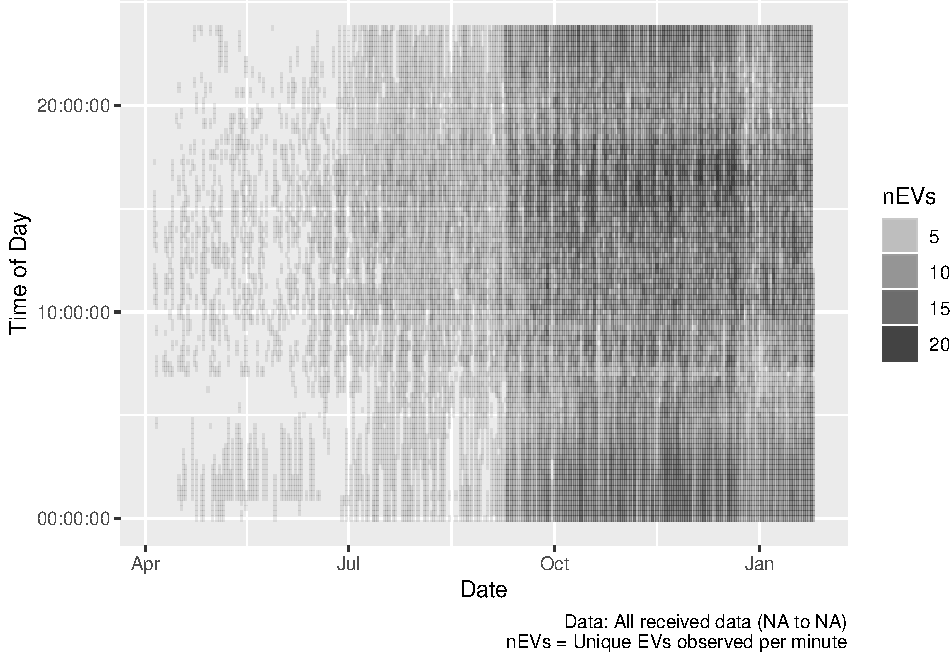
\includegraphics{/Users/ben/github/cfsOtago/evAnalysis/reports/fullReport/EVBB_report_EVBB_processed_all_v1.0_20180125_files/figure-latex/initialDataChecksPlotTile-1.pdf}
\caption{(\#fig:initialDataChecksPlotTile)Number of unique EVs observed by time of day and date}
\end{figure}

Figure @ref(fig:initialDataChecksPlotDate) shows the unique number of EVs recorded on each day and reflects the period over which Flip The Fleet installed the data collection boxes.

\begin{figure}
\centering
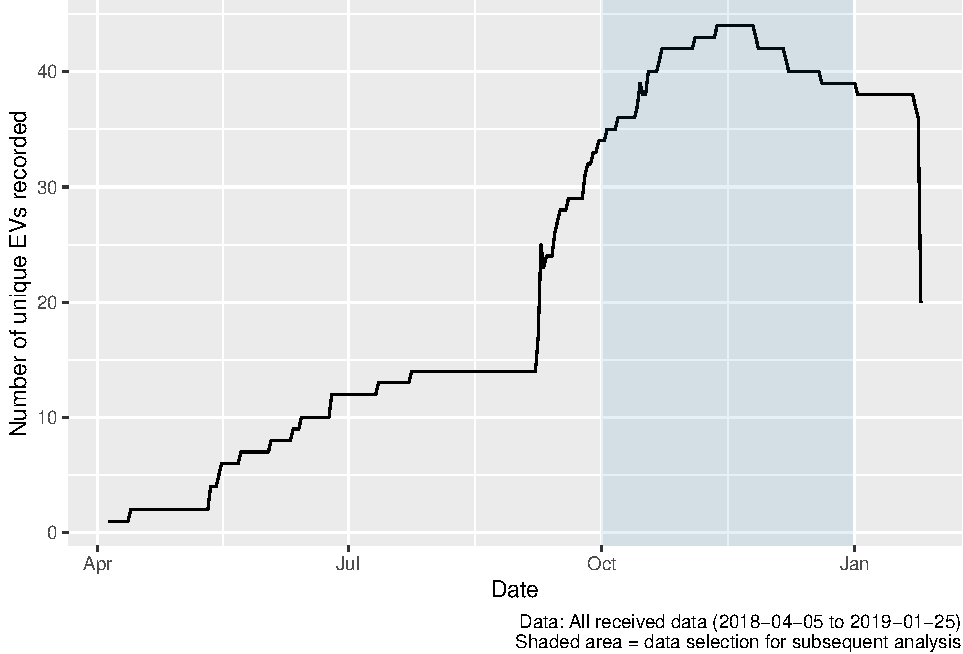
\includegraphics{/Users/ben/github/cfsOtago/evAnalysis/reports/fullReport/EVBB_report_EVBB_processed_all_v1.0_20180125_files/figure-latex/initialDataChecksPlotDate-1.pdf}
\caption{(\#fig:initialDataChecksPlotDate)Number of unique EVs observed by time of day and date}
\end{figure}

Finally, @ref(tab:noObsEVs) shows that a small number of EVs have very few observations, in some cases not extending beyond 1 day (shown as 0 days observed).

\begin{table}[t]

\caption{(\#tab:noObsEVs)Number of observations and start/end dates for vehicles (6 most scarce)}
\centering
\begin{tabular}{l|r|l|l|r|r|l}
\hline
id & nObs & startTime & endTime & meanWhCharging & maxWhCharging & nDaysObserved\\
\hline
0cc746a3f5ae75ee94068a8354b6be08 & 3 & 2018-09-09 10:46:30 & 2018-09-09 10:48:42 & 0.0000000 & 0.000000 & 0 days\\
\hline
01583b8a5f0344cc4aa3b3939a27af2a & 4 & 2018-09-09 10:34:12 & 2018-09-09 10:36:25 & 0.0000000 & 0.000000 & 0 days\\
\hline
4a6bb6e7ffc28d9d8eda7b4c6377a027 & 19 & 2018-09-08 08:48:38 & 2018-09-09 10:27:50 & 4.2251742 & 27.557201 & 1 days\\
\hline
126c8759ec95ba40070b16a11fe0e587 & 258 & 2018-09-30 11:54:18 & 2018-09-30 19:24:05 & 1.5869526 & 1.960213 & 0 days\\
\hline
4e48f4155c29c763ffe6d9e17a495200 & 530 & 2019-01-17 14:12:57 & 2019-01-25 10:31:16 & 0.0000000 & 0.000000 & 8 days\\
\hline
6e3293c77f562262ed6608db1b596d36 & 4315 & 2018-05-15 14:48:15 & 2018-12-06 13:25:56 & 0.2872577 & 47.245786 & 205 days\\
\hline
\end{tabular}
\end{table}

Taking all of the above into account we have therefore discarded:

\begin{itemize}
\tightlist
\item
  the 6 vehicles that had no recorded \emph{charging} observations (this also discarded those with very few observations - see Table @ref(tab:noObsEVs));
\item
  45 instances of charging power greater than 120kW. These were considered anomalies and as these exceed the capacity of the highest charging stations currently available in New Zealand ({\textbf{???}});
\item
  53 instances of battery state of charge observations of greater than 100\%;
\item
  all observations collected before 1st October and after 1st January in order to focus analysis on the periods with most EVs present in the data. It is hoped that this will reduce the extent to which the charging behaviour of a small number of EV owners will skew the aggregated results.
\end{itemize}

This left 45 remaining vehicles, and 941,415 observations as shown in Table @ref(tab:finalTable).

\begin{table}[t]

\caption{(\#tab:finalTable)Number of observations by charge flag (final cleaned data)}
\centering
\begin{tabular}{l|r|r|r|r}
\hline
  & Weekdays & Weekends & NA & Sum\\
\hline
Standard charging & 467705 & 160286 & 0 & 627991\\
\hline
Rapid charging & 3724 & 1810 & 0 & 5534\\
\hline
Not charging & 246438 & 61452 & 0 & 307890\\
\hline
NA & 0 & 0 & 0 & 0\\
\hline
Sum & 717867 & 223548 & 0 & 941415\\
\hline
\end{tabular}
\end{table}

\hypertarget{definitions}{%
\subsection{Definitions and preparation}\label{definitions}}

\hypertarget{chargeType}{%
\subsubsection{Charge type}\label{chargeType}}

Charging data has been broadly separated into two separate categories, `Standard' and `Rapid'. Standard charging is defined to be when the charger is reading less than 7kW - this is considered the upper limit of ordinary home charging without an expensive wiring upgrade ({\textbf{???}}). Rapid charging is defined as all charging equal to or greater than 7kW, and would likely occur at designated and purpose-built public charging stations.

It should be noted that this method is not always accurate since we can identify apparent sequences of charging which start at \textgreater{} 7kW and decline to \textless{} 7kW over a relatively short period or vice versa (see Section @ref(chargeFlagTest)). In this circumstance the first observation will be correctly classified as `Rapid' but the lower observations, which we assume are lower power `top-ups' at the end of a rapid charge will be incorrectly classified as `Standard'. As an example, we know that there are 73 sequences of charging events (out of a total of 12060) where the first and last charge types do not match.

This is clarified and corrected in Section @ref(codeSequences) for charging begin/end pairs (and thus in the results that use this data) but has yet to be resolved in other sections which use all charging observations. As a result we may currently be \emph{under-estimating} the number of rapid charge observations and \emph{over-estimating} the mean power demand of standard charges where we conduct analysis using all charging observations.

Figure @ref(fig:obsPower) shows the distribution of observed charging kW demand by inferred charge type without correcting for potential mis-classifications. Setting aside the small number of potential misclassifications noted above, the plot confirms the validity of our definition and shows that rapid charges were relatively rare in the dataset. rapid charges have two distinct power demand `peaks' at \textasciitilde{}22kW and \textasciitilde{}45kW while the far more common standard charging was mostly concentrated around 1.8kW and 3kW, with a smaller concentration around 6kW.

\begin{figure}
\centering
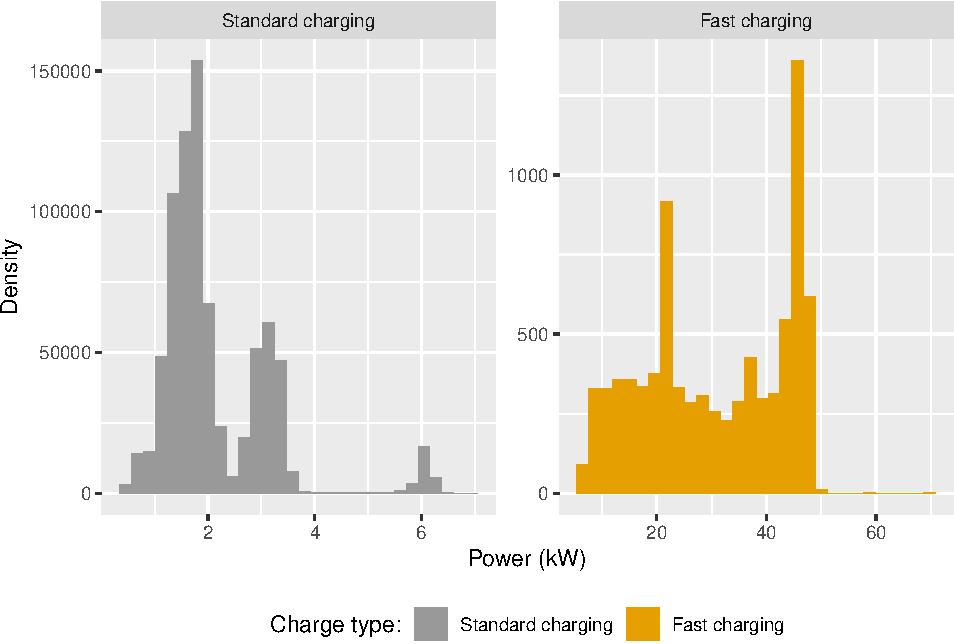
\includegraphics{/Users/ben/github/cfsOtago/evAnalysis/reports/fullReport/EVBB_report_EVBB_processed_all_v1.0_20180125_files/figure-latex/obsPower-1.pdf}
\caption{(\#fig:obsPower)Observed power demand distribution by charge type where charging observed}
\end{figure}

\hypertarget{codeSequences}{%
\subsubsection{Charge sequences}\label{codeSequences}}

In order to determine charging durations, we have identified and extracted observations which are the start and end of charging sequences. This is done using the following logic:

\begin{itemize}
\tightlist
\item
  rows were coded as ``charging begins'' if the charging power was greater than zero and the previous and following row's charging power were (respectively) equal to zero and greater than zero;
\item
  rows were coded as ``charge ends'' if the charging power was greater than zero and the previous and following row's charging power were (respectively) greater than zero and equal to zero;
\item
  rows were coded as ``charge in a sequence'' if charging power \textgreater{} 0 and the observations either side were also \textgreater{} 0
\item
  rows were coded as ``single charge events'' if charging power \textgreater{} 0 but the observations either side were 0.
\end{itemize}

\begin{table}[t]

\caption{(\#tab:seqCodeTable)Charge sequence coding results (all cleaned data)}
\centering
\begin{tabular}{l|r|r|r|r|r}
\hline
  & Standard charging & Rapid charging & Not charging & NA & Sum\\
\hline
Charging in a seq & 612644 & 4862 & 0 & 0 & 617506\\
\hline
First charge obs in a seq & 5717 & 310 & 0 & 0 & 6027\\
\hline
Last charge in a seq & 5770 & 263 & 0 & 0 & 6033\\
\hline
Not charging (0 kW) & 0 & 0 & 307890 & 0 & 307890\\
\hline
Single charge observation & 3858 & 98 & 0 & 0 & 3956\\
\hline
NA & 2 & 1 & 0 & 0 & 3\\
\hline
Sum & 627991 & 5534 & 307890 & 0 & 941415\\
\hline
\end{tabular}
\end{table}

Table @ref(tab:seqCodeTable) shows the results of this coding for all clean observations within the selected dates (2018-10-01 - 2018-12-31). As we can see most observations were coded using this scheme and we obtained 6,027 instances of charging starting, and 6,033 instances of charge ending. The additional 6 instances of charge ending than there are of the charge beginning may be due to the first (or last) instance of data collection occurring during mid-charge for some vehicles.

An alternative classification method, tested in Section @ref(chargeFlagTest), added a 120 second maximim threshold to sequences of observations but was not used as it failed to identify sparse sequences of charging events.

Comparison of the begining and end charge types showed, as suspected, that a number of pairs had mis-matching charge-types (see Table @ref(tab:checkChargeTypeErrors)). In all cases charge type was set to `Rapid' if either of the start or end observations was classified as `Rapid'. However this correction has only been made with the extracted pairs data and how not yet been applied to the full `all observations' data.

\begin{table}[t]

\caption{(\#tab:checkChargeTypeErrors)Charge type errors detected via mis-matching start and end observations vs uncorrected charge type}
\centering
\begin{tabular}{l|r|r|r|r}
\hline
  & Standard charging & Rapid charging & Not charging & Sum\\
\hline
Error: first = Rapid, last = Standard & 0 & 60 & 0 & 60\\
\hline
Error: first = Standard, last = Rapid & 13 & 0 & 0 & 13\\
\hline
OK: first = Rapid, last = Rapid & 0 & 250 & 0 & 250\\
\hline
OK: first = Standard, last = Standard & 5704 & 0 & 0 & 5704\\
\hline
Sum & 5717 & 310 & 0 & 6027\\
\hline
\end{tabular}
\end{table}

The charge duration was then calculated as being the time duration between each pair of `first in charge sequence' and `last in charge sequence' observations.

Figure @ref(fig:durationHist) shows the overall distribution of all charging sequences using the corrected charge type. Clearly there are very small and a few very large values for both charging types.

\begin{figure}
\centering
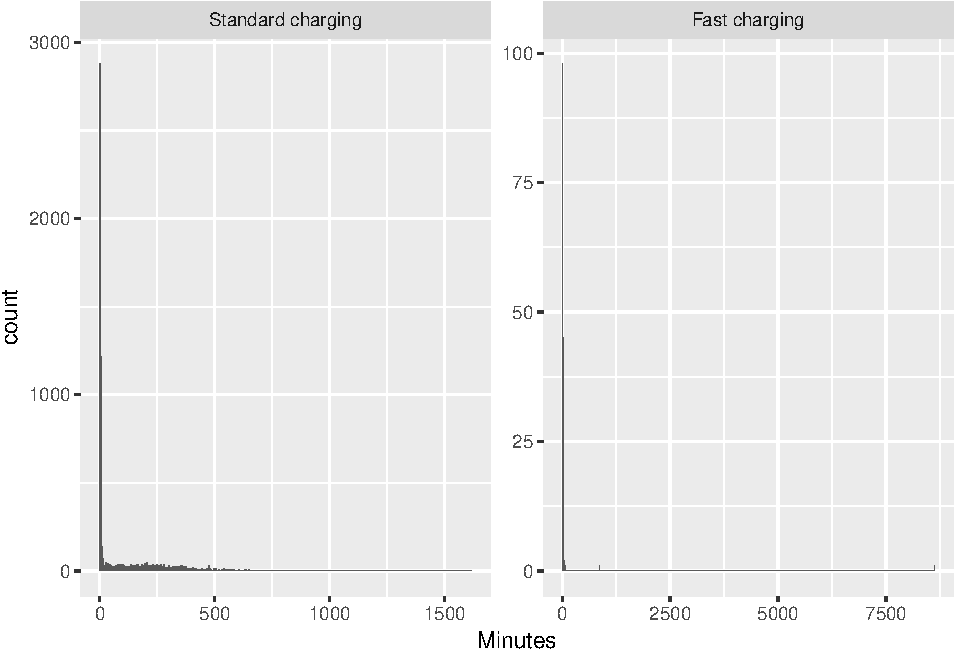
\includegraphics{/Users/ben/github/cfsOtago/evAnalysis/reports/fullReport/EVBB_report_EVBB_processed_all_v1.0_20180125_files/figure-latex/durationHist-1.pdf}
\caption{(\#fig:durationHist)Duration of charging sequences by corrected charge type}
\end{figure}

Table @ref(tab:durationDescTable) shows the overall distributions and indicates the extent to which the means are skewed by the very small and a few very large values shown in Figure @ref(fig:durationHist).

\begin{table}[t]

\caption{(\#tab:durationDescTable)Duration of all charge sequences by charge type}
\centering
\begin{tabular}{l|r|l|r|l|l}
\hline
chargeTypeCorrected & N & mean & median & min & max\\
\hline
Standard charging & 5702 & 97.38 mins & 3.38 & 0.27 mins & 1442.3 mins\\
\hline
Rapid charging & 323 & 23.16 mins & 14.27 & 0.02 mins & 865.7 mins\\
\hline
\end{tabular}
\end{table}

Table @ref(tab:durationLongTableStd) shows the longest duration `standard' charge events while Table @ref(tab:durationLongTableRapid) shows the longest duration `Rapid' charge events.

\begin{table}[t]

\caption{(\#tab:durationLongTableStd)Duration of longest charge sequences (Standard charging)}
\centering
\begin{tabular}{l|l|l|l|l|l|r}
\hline
dvID & startTime & day\_of\_week & chargeType & chargeTypeCorrected & pairDuration & duration\_hours\\
\hline
Vehicle 27 & 02:54:06 & Mon & Standard charging & Standard charging & 1442.30 mins & 24.04\\
\hline
Vehicle 32 & 11:28:58 & Sat & Standard charging & Standard charging & 1353.40 mins & 22.56\\
\hline
Vehicle 37 & 06:40:33 & Fri & Standard charging & Standard charging & 1341.80 mins & 22.36\\
\hline
Vehicle 37 & 23:44:13 & Sun & Standard charging & Standard charging & 1324.10 mins & 22.07\\
\hline
Vehicle 37 & 05:54:34 & Thu & Standard charging & Standard charging & 1264.10 mins & 21.07\\
\hline
Vehicle 18 & 02:37:53 & Thu & Standard charging & Standard charging & 1228.23 mins & 20.47\\
\hline
Vehicle 32 & 15:31:56 & Sun & Standard charging & Standard charging & 1125.35 mins & 18.76\\
\hline
Vehicle 37 & 04:35:00 & Fri & Standard charging & Standard charging & 1063.82 mins & 17.73\\
\hline
Vehicle 5 & 02:41:37 & Sun & Standard charging & Standard charging & 1034.12 mins & 17.24\\
\hline
Vehicle 29 & 03:20:28 & Sat & Standard charging & Standard charging & 999.90 mins & 16.66\\
\hline
\end{tabular}
\end{table}

\begin{table}[t]

\caption{(\#tab:durationLongTableRapid)Duration of longest charge sequences (Rapid charging)}
\centering
\begin{tabular}{l|l|l|l|l|l|r}
\hline
dvID & startTime & day\_of\_week & chargeType & chargeTypeCorrected & pairDuration & duration\_hours\\
\hline
Vehicle 34 & 06:10:19 & Wed & Standard charging & Rapid charging & 865.70 mins & 14.43\\
\hline
Vehicle 12 & 10:08:02 & Thu & Rapid charging & Rapid charging & 582.53 mins & 9.71\\
\hline
Vehicle 38 & 01:37:03 & Thu & Rapid charging & Rapid charging & 398.27 mins & 6.64\\
\hline
Vehicle 41 & 04:39:24 & Tue & Rapid charging & Rapid charging & 227.85 mins & 3.80\\
\hline
Vehicle 1 & 20:20:46 & Thu & Rapid charging & Rapid charging & 173.58 mins & 2.89\\
\hline
Vehicle 47 & 01:40:40 & Tue & Rapid charging & Rapid charging & 116.37 mins & 1.94\\
\hline
Vehicle 21 & 09:04:03 & Sun & Rapid charging & Rapid charging & 90.57 mins & 1.51\\
\hline
Vehicle 42 & 05:02:37 & Mon & Standard charging & Rapid charging & 80.27 mins & 1.34\\
\hline
Vehicle 33 & 05:23:22 & Sat & Rapid charging & Rapid charging & 50.43 mins & 0.84\\
\hline
Vehicle 1 & 03:59:40 & Thu & Rapid charging & Rapid charging & 49.83 mins & 0.83\\
\hline
\end{tabular}
\end{table}

Figure @ref(fig:shortDuration) shows the distribution of very short charging sequences. As we can see these appear to be generally less than 8 minutes in length for Standard Charges.

\begin{figure}
\centering
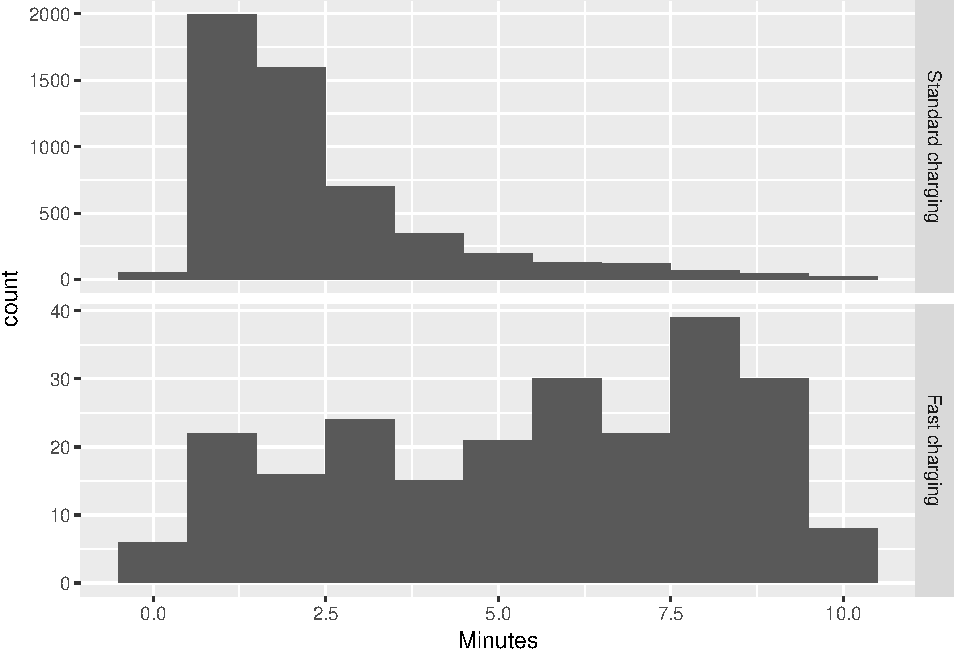
\includegraphics{/Users/ben/github/cfsOtago/evAnalysis/reports/fullReport/EVBB_report_EVBB_processed_all_v1.0_20180125_files/figure-latex/shortDuration-1.pdf}
\caption{(\#fig:shortDuration)Duration of charging sequences \textless{} 15 minutes}
\end{figure}

Manual inspection of the data showed that these short-duration `standard' charging events generally occurred near the end of a longer-duration charging sequence. It appeared that once the vehicle had reached its highest state of charge, charging would intermittently stop and start again. This is probably due to the behaviour of the charger once the battery was almost full.

Table @ref(tab:durationDescTableReduced) repeats the same descriptive statistics reported in Table @ref(tab:durationDescTable) but for all sequences of greater than 8 minute duration. We can now see that the mean and median durations for both Standard and Rapid Charge sequences are closer.

\begin{table}[t]

\caption{(\#tab:durationDescTableReduced)Duration of charge sequences > 8 minutes by charge type (minutes)}
\centering
\begin{tabular}{l|r|l|r|l|l}
\hline
chargeTypeCorrected & N & mean & median & min & max\\
\hline
Standard charging & 2244 & 244.11 mins & 210.10 & 8.03 mins & 1442.3 mins\\
\hline
Rapid charging & 235 & 30.46 mins & 18.22 & 8.12 mins & 865.7 mins\\
\hline
\end{tabular}
\end{table}

In addition to the many `short' charging duration values, a small number of unreasonably long charging durations (longer than 14 hours for rapid charging - see Table @ref(tab:durationLongTableRapid)) were calculated. As these exceeded the expected charge durations of even the highest capacity vehicles currently available, they were also assumed to be anomalies. The analyses in Section @ref(duration) below was therefore made with the following charge events excluded from the data:

\begin{itemize}
\tightlist
\item
  duration \textless{} 8 minutes for standard charging (3458 observations - noting that some of these may be short low power `Rapid charge' events as discussed in Section @ref(chargeType))
\item
  duration \textgreater{} 840 minutes (14 hours) for rapid charging (1 observations)
\end{itemize}

Figure @ref(fig:longDuration) shows the distribution of charging sequences with the excessively long or short events removed. These charging durations appear more reasonable when considering standard battery capacities and available charge power.

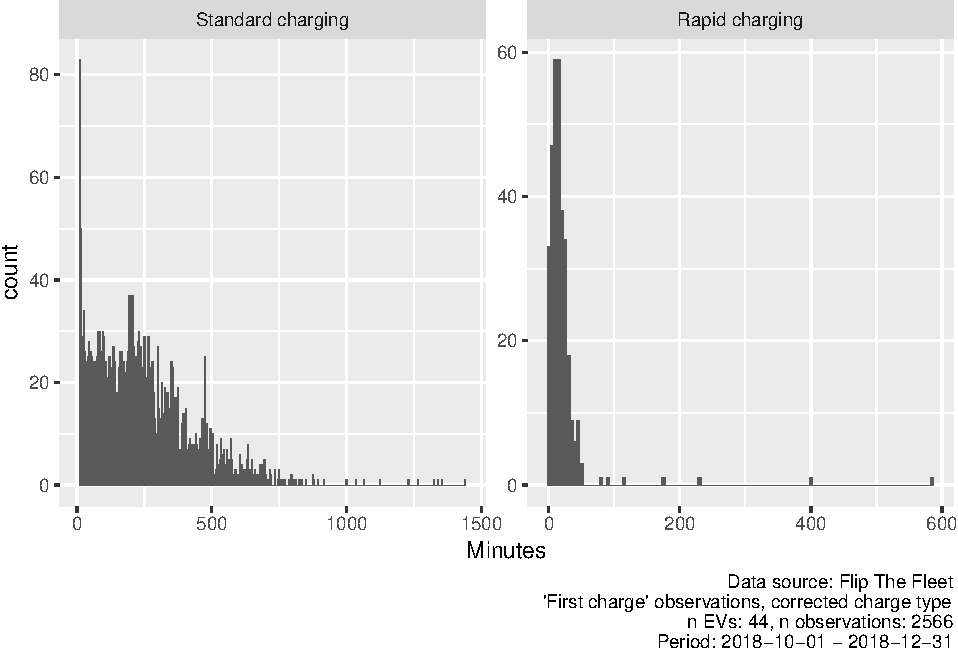
\includegraphics{/Users/ben/github/cfsOtago/evAnalysis/reports/fullReport/EVBB_report_EVBB_processed_all_v1.0_20180125_files/figure-latex/longDuration-1.pdf}

\begin{table}[t]

\caption{(\#tab:longDuration)Duration of charge sequences, final duration data}
\centering
\begin{tabular}{l|r|l|r|l|l}
\hline
chargeTypeCorrected & N & mean & median & min & max\\
\hline
Standard charging & 2244 & 244.11 mins & 210.10 & 8.03 mins & 1442.30 mins\\
\hline
Rapid charging & 322 & 20.54 mins & 14.26 & 0.02 mins & 582.53 mins\\
\hline
\end{tabular}
\end{table}

\hypertarget{results}{%
\section{Results}\label{results}}

\hypertarget{time-of-charging}{%
\subsection{Time of charging}\label{time-of-charging}}

It has been suggested that EV charging is more likely to occur in the early evening when drivers return from daily commutes or school pick-ups ({\textbf{???}}).

Figure @ref(fig:chargeTimeProp) plots the distribution of each charge type over time of day and confirms the very low incidence of rapid charging. It also supports the suggestion that standard charging (at home) does not appear to begin until later in the evening.

\begin{figure}
\centering
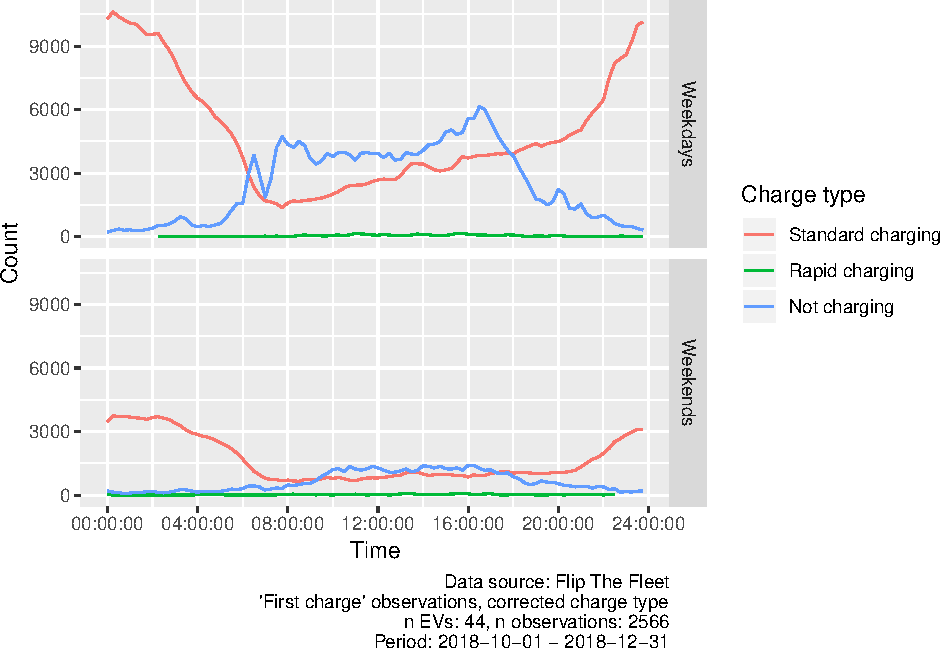
\includegraphics{/Users/ben/github/cfsOtago/evAnalysis/reports/fullReport/EVBB_report_EVBB_processed_all_v1.0_20180125_files/figure-latex/chargeTimeProp-1.pdf}
\caption{(\#fig:chargeTimeProp)Density plot of charging start times during weekdays}
\end{figure}

Figure @ref(fig:chargeTimeTypes) extends this analysis by showing charging and non-charging observations at different times of day by weekday vs weekends using a density plot to show releative distributions over time within each type. The plot clearly shows non-charging during day-time use and also shows a bi-model distribution for rapid charging (non-corrected categorisation). Standard charging also shows a bi-modal distribution with a peak around 22:00 on weekdays and another at 01:00 presumably indicating the use of timed or `smart' charging or trickle events.

\begin{figure}
\centering
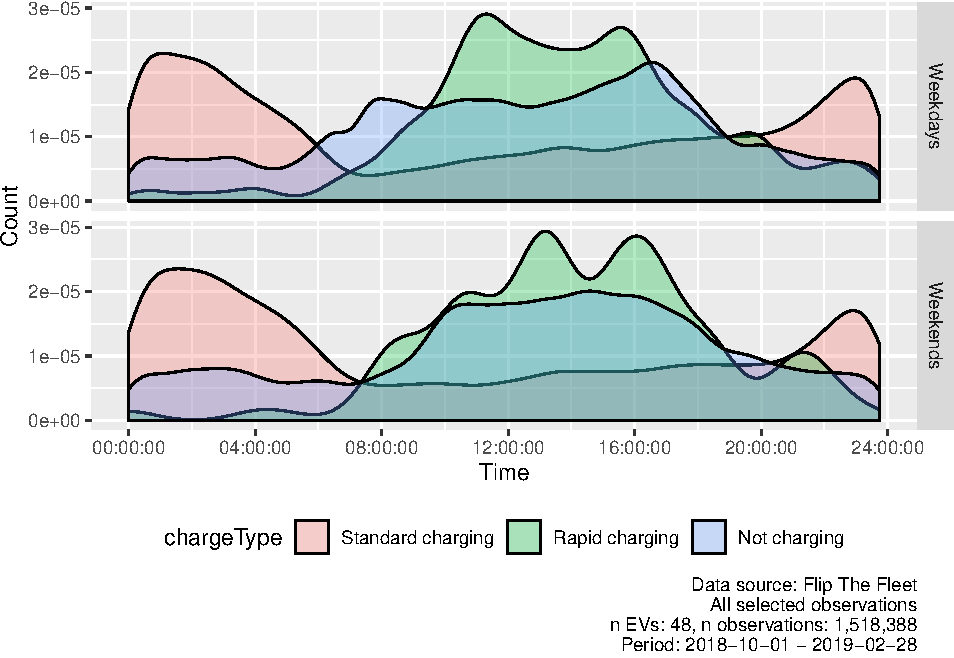
\includegraphics{/Users/ben/github/cfsOtago/evAnalysis/reports/fullReport/EVBB_report_EVBB_processed_all_v1.0_20180125_files/figure-latex/chargeTimeTypes-1.pdf}
\caption{(\#fig:chargeTimeTypes)Density plot of charging start times during weekdays}
\end{figure}

In general, these results indicate that the greatest frequency of standard charging events occurs between 20:00 and 08:00, with very low occurrences of charging during morning and evening grid peaks. Rapid charging on the other hand is a day-time activity on both weekdays and weekends.

To make the patterns of `initial charging' clearer, we use just the `first' charge observation in a pair (see above) and also exclude automatic battery `top-ups' (refer to Section @ref(SoC)) by filtering out any data where a charging observation begins while the state of charge is greater than 90\%. Having done so, Figure @ref(fig:chargeBeginsTimeLine) shows the distribution of the start of `charge sequences' and shows that the number of charging event starts increases steadily through the day before an apparent brief lull between 19:00 and 21:00 and then increases substantially thereafter.

\begin{figure}
\centering
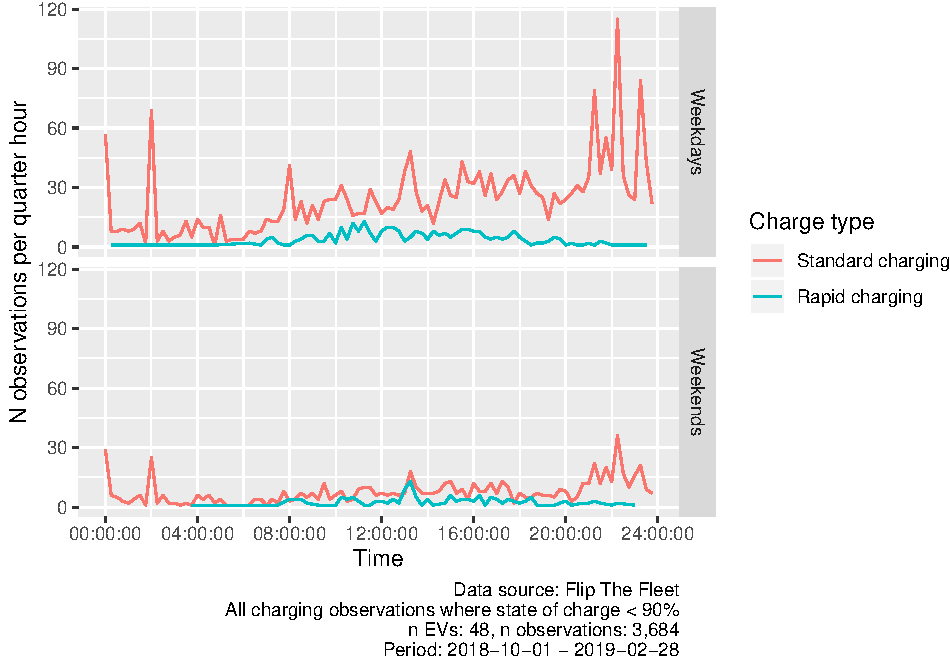
\includegraphics{/Users/ben/github/cfsOtago/evAnalysis/reports/fullReport/EVBB_report_EVBB_processed_all_v1.0_20180125_files/figure-latex/chargeBeginsTimeLine-1.pdf}
\caption{(\#fig:chargeBeginsTimeLine)Charging start times where state of charge \textless{} 90\%}
\end{figure}

Figure @ref(fig:chargeBeginsTimeDensity) uses a density plot to represent the proportion of charging sequences that start at different times of the day on weekdays vs weekends for standard and rapid charging (corrected classification).

\begin{figure}
\centering
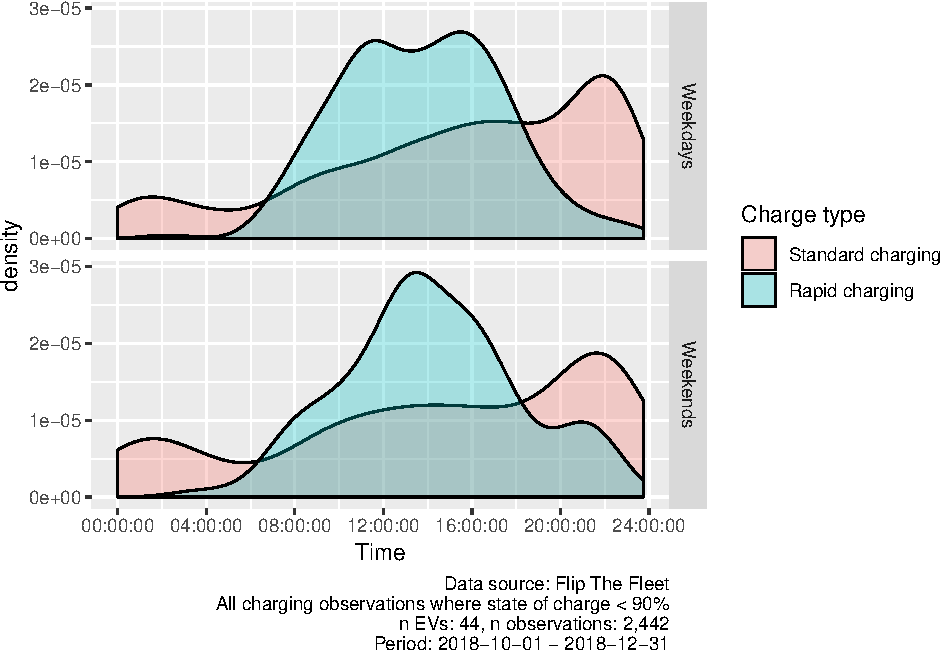
\includegraphics{/Users/ben/github/cfsOtago/evAnalysis/reports/fullReport/EVBB_report_EVBB_processed_all_v1.0_20180125_files/figure-latex/chargeBeginsTimeDensity-1.pdf}
\caption{(\#fig:chargeBeginsTimeDensity)Density plot of charging start times where state of charge \textless{} 90\%}
\end{figure}

As we can see, standard charging sequences (as opposed to single observations) have a noticeably different profile to charging patterns for rapid charges. It suggests that the largest number of standard charging events start between 20:00 and 22:00 and run overnight, and perhaps use the more powerful public charge points to top up during the day. However the plot also show a substantial proportion of charging events start earlier in the day, including during the NZ \href{https://www.electrickiwi.co.nz/hour-of-power}{peak demand periods} of 07:00 - 09:00 and 17:00 - 21:00.

Standard charging events were most likely to begin around 10pm during both weekdays and weekends. As it seems unlikely that this is due to vehicle drivers returning home at this hour, this effect may be due to drivers setting the charger on a timer to take advantage of cheaper ``off-peak'' electricity times, which frequently begin around 10pm.

Rapid charging events were most likely to begin at 11:30am on weekdays and 1pm during weekends.

\hypertarget{patterns-of-power-demand}{%
\subsection{Patterns of power demand}\label{patterns-of-power-demand}}

Given this distribution of charging events, it is important to understand their magnitude to understand the potential effect on the electricity network. Although we are hampered by the lack of observations when the EV is inactive, this section analyses the patterns of power demand for the observations we have.

Overall 75\% of standard charging observations were 1.45 kW or more but the figure was 20.05 kW or more for rapid charging.

Figure @ref(fig:nonRapidPowerPlotDT) shows the mean charging demand in kW calculated across all observations after setting rapid charge observations to 0 kW. As we would expect the kW load due to the EVs follows essentially the same shape as the charging event proportions shown above but with slightly more evidence of a 13:00 and 16:00 mini-peak and distinct differences between weekday and weekend mornings. As before, the apparent rapid increase in demand (and the pre-20:00 spike) are more likely to be due to decreasing numbers of `non-charging' observations than increases in charging (see Figure @ref(fig:chargeTimeTypes).

\begin{figure}
\centering
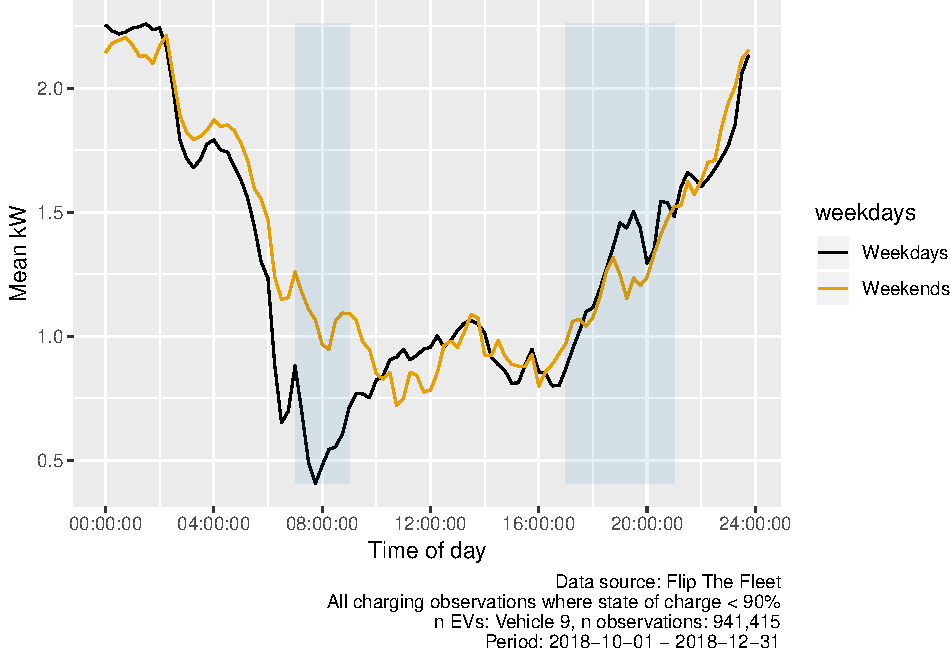
\includegraphics{/Users/ben/github/cfsOtago/evAnalysis/reports/fullReport/EVBB_report_EVBB_processed_all_v1.0_20180125_files/figure-latex/nonRapidPowerPlotDT-1.pdf}
\caption{(\#fig:nonRapidPowerPlotDT)Mean kW per quarter hour (treating rapid charging as 0 kW)}
\end{figure}

Figure @ref(fig:rapidPowerPlotDT) repeats this analysis but shows the mean charging demand in kW calculated across all observations after setting standard charge observations to 0 kW. Again, the kW load due to the EVs follows essentially the same shape as the charging event counts shown above and the low mean value should remind us that rapid charging was relatively rare in the data.

\begin{figure}
\centering
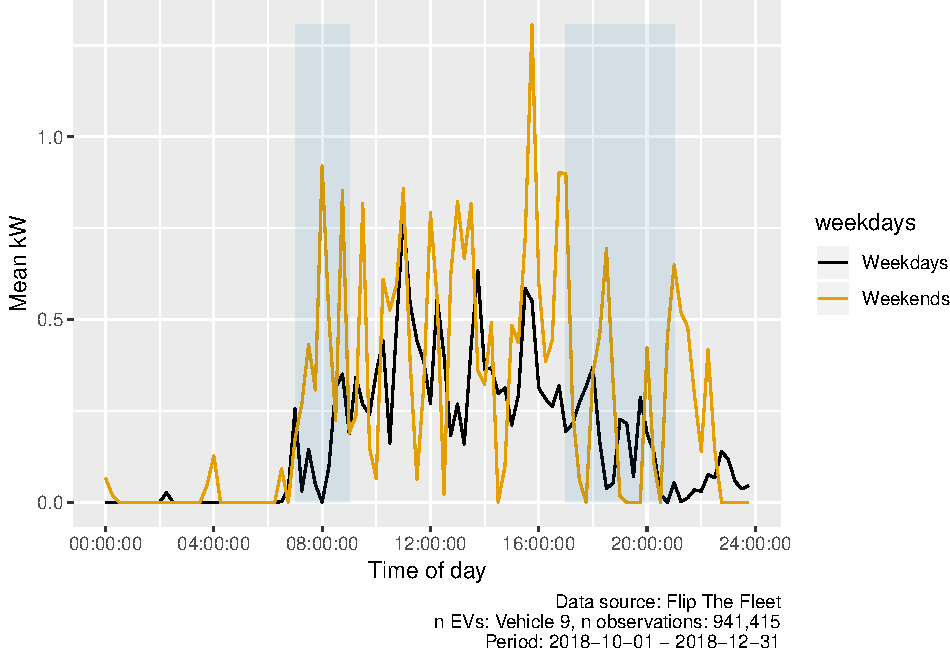
\includegraphics{/Users/ben/github/cfsOtago/evAnalysis/reports/fullReport/EVBB_report_EVBB_processed_all_v1.0_20180125_files/figure-latex/rapidPowerPlotDT-1.pdf}
\caption{(\#fig:rapidPowerPlotDT)Mean kW per quarter hour (treating standard charging as 0 kW)}
\end{figure}

In next plots we use transparency to indicate the number of EVs contributing to each of the mean calculations to give a guide to their reliability and indicate the relative proportion of sample EVs that contribute to each mean value. Dots with stronger colours indicate means calculated from a larger number of EVs and, given the data gaps noted in Section @ref(background), this therefore indicates patterns which are generally shared across a larger number of EVs. We would therefore expect darker dots (most vehicles) durng overnight charge times and lighter plots (fewer vehicles co-incidentally charging) through the day.

Figure @ref(fig:meanChargeByTimeStd) shows the mean power demand for standard charging observations by time of day and weekdays vs weekends for the selected time period. This plot appears to show that there are three peaks in standard charging, one at 10:00, one at 18:00 (possibly based on fewer EVs) and one after midnight on weekdays. There are also noticeable 07:00 and 16:00 charging blips. On the other hand at weekends the daytime peak shifts to 14:00. Thus, while our previous analysis suggested that charging events were more likely to start later in the evening, the power demand of earlier charging events may actually be relatively high and co-incide with existing peak demand periods.

\begin{figure}
\centering
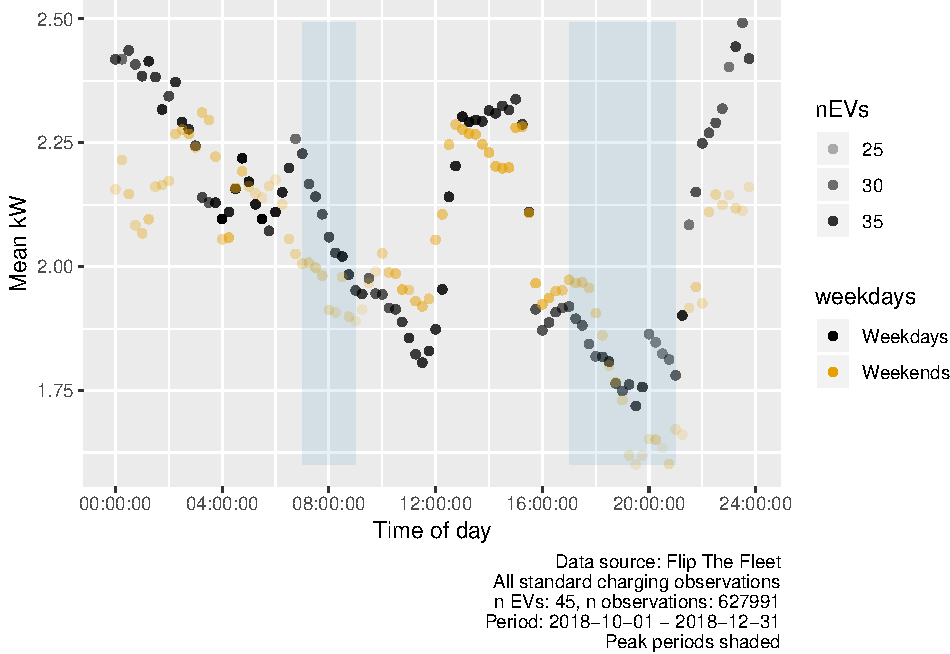
\includegraphics{/Users/ben/github/cfsOtago/evAnalysis/reports/fullReport/EVBB_report_EVBB_processed_all_v1.0_20180125_files/figure-latex/meanChargeByTimeStd-1.pdf}
\caption{(\#fig:meanChargeByTimeStd)Mean charging power demand (kW) by time of day (`standard' charging)}
\end{figure}

Rapid charging however has no detectable pattern other than a clear increase in density during weekday daytimes (Figure @ref(fig:meanChargeByTimeRapid)). However, we can now see the effect that rapid charging may have with significant EV uptake.

\begin{figure}
\centering
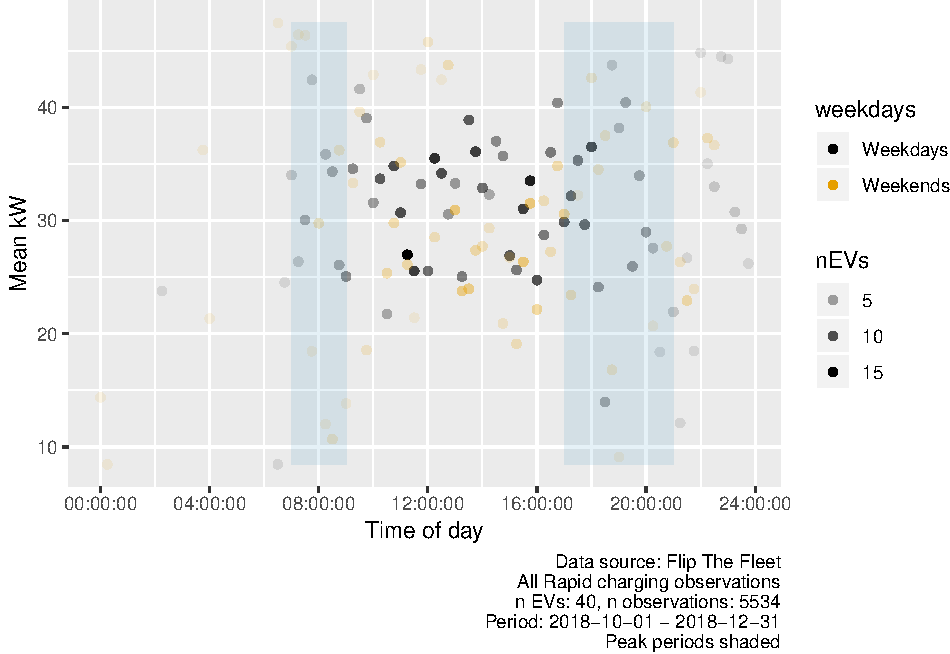
\includegraphics{/Users/ben/github/cfsOtago/evAnalysis/reports/fullReport/EVBB_report_EVBB_processed_all_v1.0_20180125_files/figure-latex/meanChargeByTimeRapid-1.pdf}
\caption{(\#fig:meanChargeByTimeRapid)Mean charging power demand (kW) by time of day (`rapid' charging)}
\end{figure}

It is possible that the `standard charge' day-time peak is skewed by mis-classified short low power `Rapid charge' observations (see Section @ref(chargeType)). Figure @ref(fig:medianChargeByTime) attempts to allow for this misclassification by plotting the median rather than the mean. The plot more clearly shows the 10:00 weekday spike which, if we assume that the mis-classified `Rapid charges' will be skewing the standard charge mean value upwards, is likely to be due to mis-classified `Rapid charging'. However the 18:00 peak persists as does the 14:00 weekend peak while overnight charging levels are relatively stable as we would expect from @ref(fig:meanChargeByTimeStd).

\begin{figure}
\centering
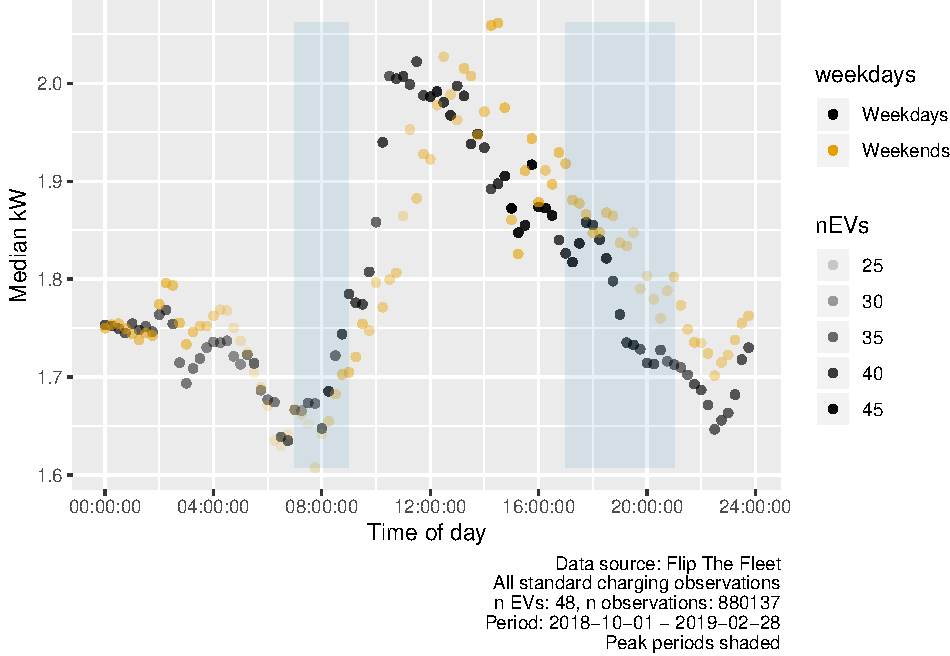
\includegraphics{/Users/ben/github/cfsOtago/evAnalysis/reports/fullReport/EVBB_report_EVBB_processed_all_v1.0_20180125_files/figure-latex/medianChargeByTime-1.pdf}
\caption{(\#fig:medianChargeByTime)Median charging power demand (kW) by time of day}
\end{figure}

Figure @ref(fig:meanChargeByTimeMonth) repeats the median power-based analysis for `Standard charging' but shows the results by month. While the sample size is probably too small to draw robust conclusions there appear to be differences between months with December showing few discernable peaks and September and January showing much lower daytime weekday charging. In addition, weekdays and weekends are much more similar in November and December.

\begin{figure}
\centering
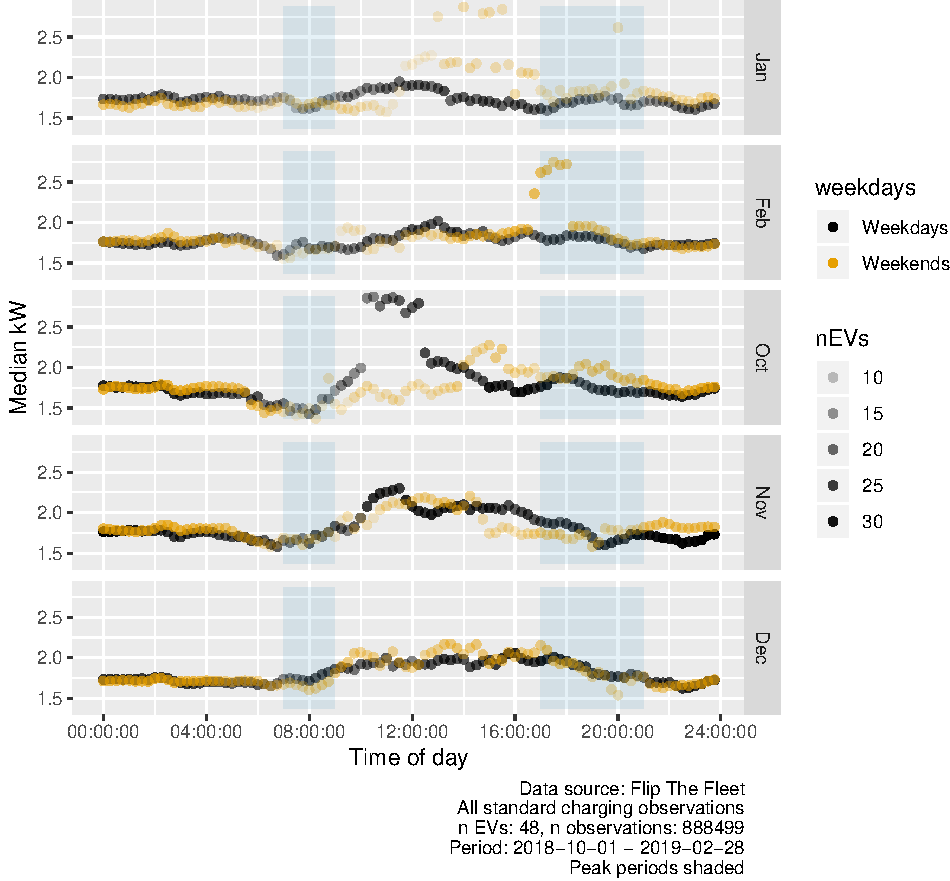
\includegraphics{/Users/ben/github/cfsOtago/evAnalysis/reports/fullReport/EVBB_report_EVBB_processed_all_v1.0_20180125_files/figure-latex/meanChargeByTimeMonth-1.pdf}
\caption{(\#fig:meanChargeByTimeMonth)Median charging power demand (kW) by time of day and month}
\end{figure}

On face value the results suggest that EVs could be placing additional power demand on local and national networks during well-known periods of peak demand although this appears to vary by month for this small sample of EV owners.

\begin{quote}
Clearly this analysis should be revisited once the potential misclassification of `rapid' as `standard' charging observations has been resolved and the `missing' non-use (zero charging) observations have been imputed.
\end{quote}

\hypertarget{duration}{%
\subsection{Charging duration}\label{duration}}

This section analyses the duration of observed charging events to understand when longer charging sequences are likely to occur. Table @ref(tab:meanDurationTable) shows the mean durations for all all charging events by event start time for standard charging durations greater than 8 minutes (see Section @ref(codeSequences)) and all rapid charging events for observations collected after 01 October 2018.

\begin{table}[t]

\caption{(\#tab:meanDurationTable)Mean duration of charge events by charge type (filtered data, corrected charge type)}
\centering
\begin{tabular}{l|l|l|l|l|r}
\hline
chargeTypeCorrected & mean & median & min & max & sd\\
\hline
Standard charging & 244.11 mins & 210.10 mins & 8.03 mins & 1442.30 mins & 186.98\\
\hline
Rapid charging & 20.54 mins & 14.26 mins & 0.02 mins & 582.53 mins & 42.86\\
\hline
\end{tabular}
\end{table}

\begin{table}[t]

\caption{(\#tab:makeDurationTimeMean)Mean duration of charge sequences (values > 480 minutes)}
\centering
\begin{tabular}{l|l|l|l|r}
\hline
qHour & chargeTypeCorrected & weekdays & meanDuration & nEVs\\
\hline
23:30:00 & Standard charging & Weekends & 1324.10 mins & 1\\
\hline
15:30:00 & Standard charging & Weekends & 528.46 mins & 4\\
\hline
15:45:00 & Standard charging & Weekends & 497.73 mins & 1\\
\hline
00:45:00 & Standard charging & Weekends & 495.30 mins & 1\\
\hline
\end{tabular}
\end{table}

Figure @ref(fig:durationTimeMean) plots the mean duration by time of day and weekday vs weekend and charge type. As before we use transparency to indicate the number of unique EVs contributing to the mean values and we have removed a small number of very large duration outliers (mean duration \textgreater{} 540 minutes or 9 hours) which appears to be based on just 1 or 2 EVs (see Table @ref:(tab:makeDurationTimeMean)).

As we would expect, the plot shows that for standard charging mean `forward' duration generally decreases from midnight, presumably as batteries are becoming fully charged through to 06:00 and then increases as the time of starting to charge increases through the day before trending downwards before midnight. Again, this confirms that charge events starting in or just after the evening peak demand period on both weekdays and weekends are likely to be longer, possibly reflecting the lower state of charge at this time of day (following use).

Duration of rapid charge events by start time appear to be more randomly distributed, although very few events were recorded between midnight and 7am. This, along with the comparatively low number of recorded rapid charge events indicated in Fig. @ref(fig:obsPower) suggests that drivers utilize rapid charging only ``as necessary'' to ensure they have enough battery capacity to complete their journey or when `at work' or conducting some other mobility related task such as shopping.

\begin{figure}
\centering
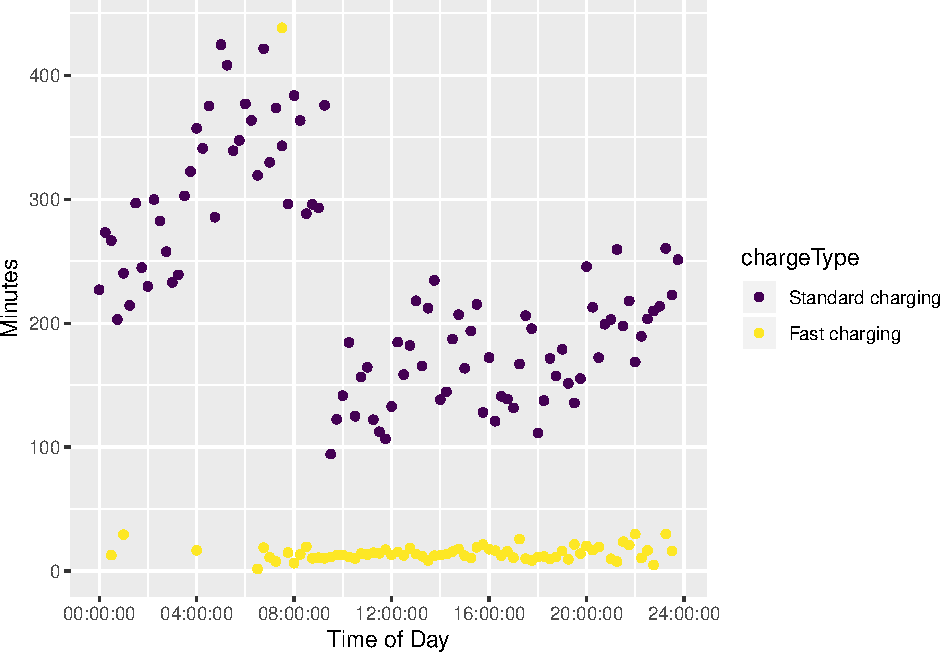
\includegraphics{/Users/ben/github/cfsOtago/evAnalysis/reports/fullReport/EVBB_report_EVBB_processed_all_v1.0_20180125_files/figure-latex/durationTimeMean-1.pdf}
\caption{(\#fig:durationTimeMean)Mean duration (within quarter hours) by time of charging start}
\end{figure}

\hypertarget{SoC}{%
\subsection{State of charge}\label{SoC}}

The state of charge is the percentage of energy still available to be used in the battery. In future, electric vehicles may be able to discharge any remaining battery charge as electricity into the grid, a process known as vehicle to grid (V2G) energy transfer. This may allow electric vehicles to have a net beneficial effect on the grid, reducing the evening peaks by providing electricity to the home during this period, and then recharging later in the evening or early the next morning when peak demand has diminished.

This section provides an indication of the state of charge of electric vehicles upon charging, so that the potential of V2G technology can be assessed.

\begin{figure}
\centering
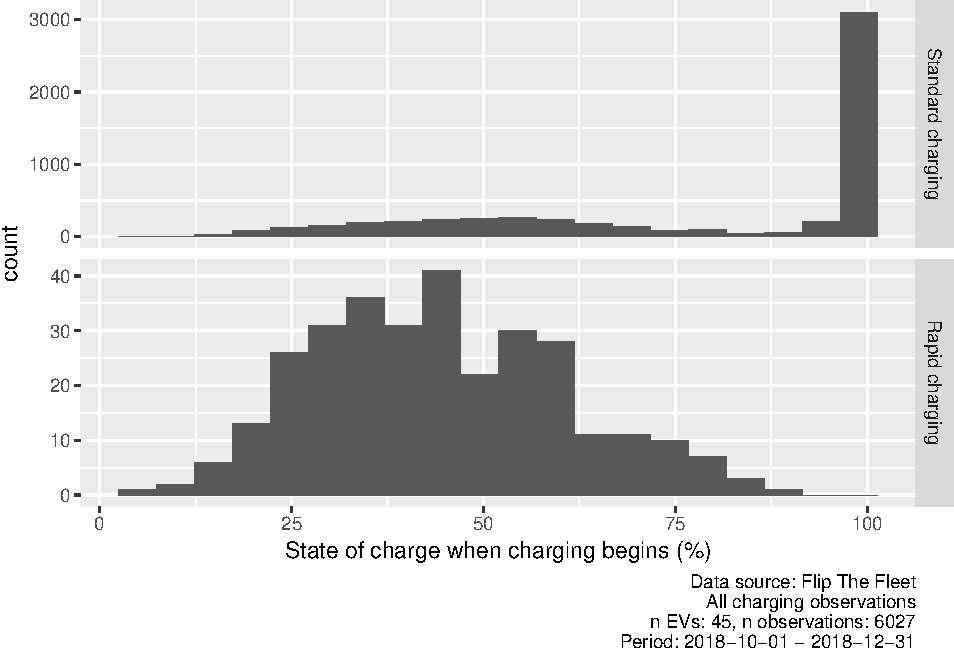
\includegraphics{/Users/ben/github/cfsOtago/evAnalysis/reports/fullReport/EVBB_report_EVBB_processed_all_v1.0_20180125_files/figure-latex/SoCplot1-1.pdf}
\caption{(\#fig:SoCplot1)Value of state of charge (all charging observations)}
\end{figure}

As can be seen in Figure @ref(fig:SoCplot1), using the cleaned complete observations data, the state of charge for the majority of standard charge observations is above 90\%. This is most likely due to the manner in which the charger regularly turns off and on again near the end of the charging cycle as described in Section @ref(cleaning).

Figure @ref(fig:SoCplot2) shows the state of charge values for all charging events but with state of charge greater than 90\% removed from the data for clarity. The figure indicates that many vehicles begin charging despite having greater than 50\% charge remaining. This has clear implications for battery life management since continually top-up charging is known to substantially shorten the lifetime of EV batteries (XX ref needed XX). However it also indicates the potential to use the charge in the battery to feed into the grid, especially in the residential context.

\begin{figure}
\centering
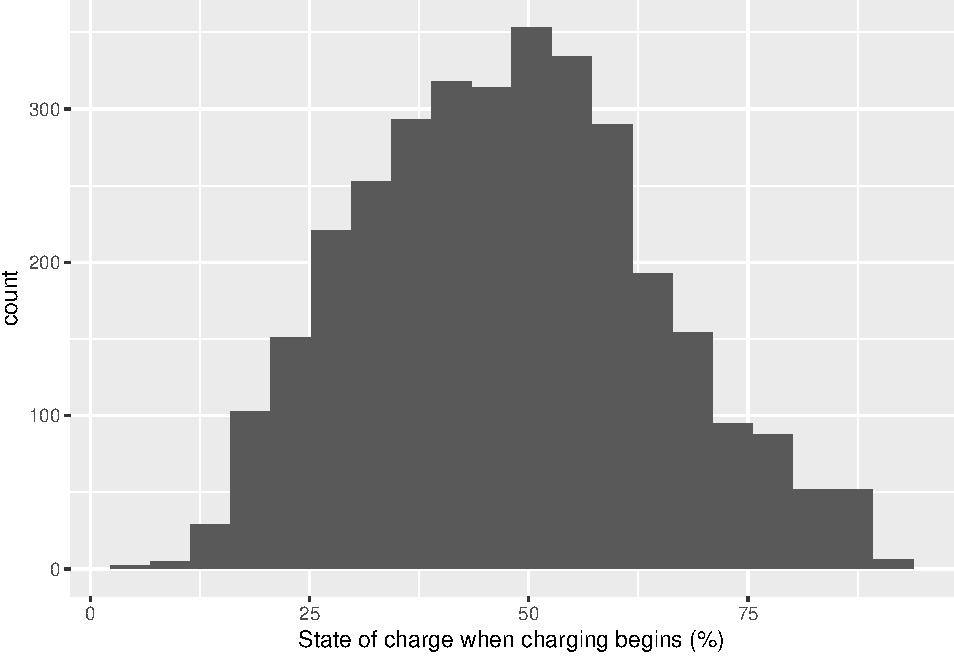
\includegraphics{/Users/ben/github/cfsOtago/evAnalysis/reports/fullReport/EVBB_report_EVBB_processed_all_v1.0_20180125_files/figure-latex/SoCplot2-1.pdf}
\caption{(\#fig:SoCplot2)Value of state of charge (values \textgreater{} 90\% removed)}
\end{figure}

Figure @ref(fig:SoCplot3) repeats this analysis but uses the cleaned and corrected inferred start/end of charging sequence data instead of all charging observations. Figure @ref(fig:SoCplot3) shows very similar distributions to the previous `all-observations' plot (Figure @ref(fig:SoCplot2)) and confirms that sequences of standard charging in particular most frequently start with battery state of charge over 50\%.

\begin{figure}
\centering
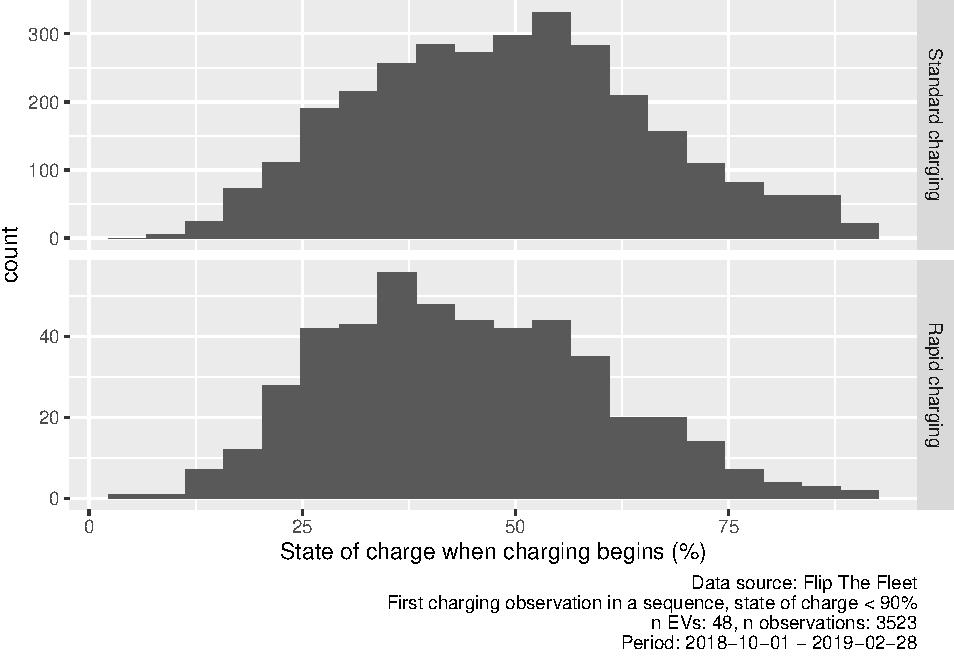
\includegraphics{/Users/ben/github/cfsOtago/evAnalysis/reports/fullReport/EVBB_report_EVBB_processed_all_v1.0_20180125_files/figure-latex/SoCplot3-1.pdf}
\caption{(\#fig:SoCplot3)Value of state of charge at beginning of charging sequence (chargeType corrected, values \textgreater{} 90\% removed)}
\end{figure}

\begin{figure}
\centering
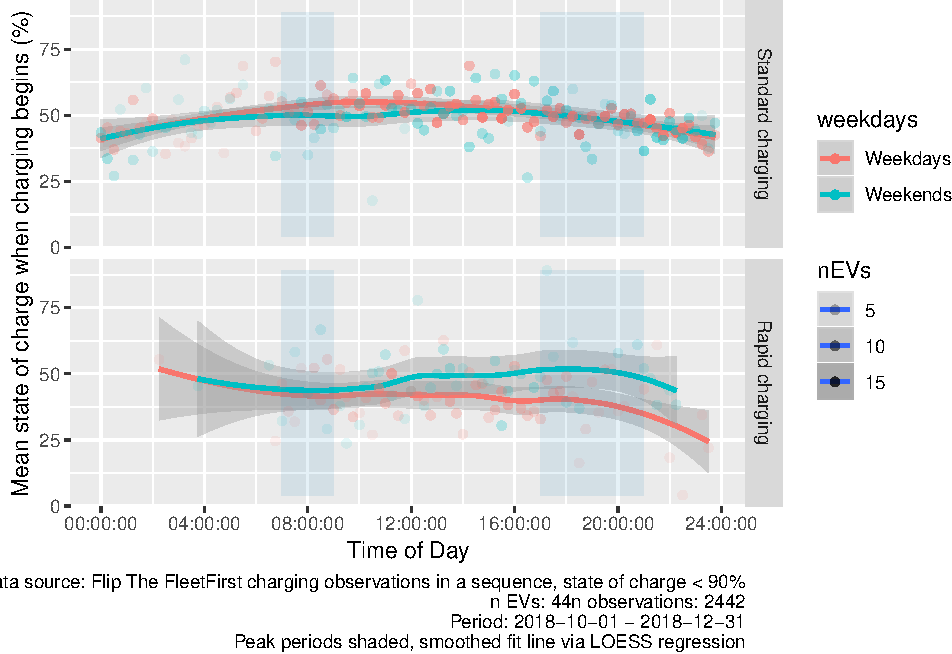
\includegraphics{/Users/ben/github/cfsOtago/evAnalysis/reports/fullReport/EVBB_report_EVBB_processed_all_v1.0_20180125_files/figure-latex/SoCplotTiming-1.pdf}
\caption{(\#fig:SoCplotTiming)Mean state of charge at beginning of charge sequence by time of day (chargeType corrected, values \textgreater{} 90\% removed)}
\end{figure}

Finally, Figure @ref(fig:SoCplotTiming) shows the mean \% charge by time of first charging observation in a sequence using the cleaned and corrected inferred start/end of charging sequence data. The plot suggests that this capacity may be relatively stable throughout the day albiet with slightly higher mean capacity around the morning peak as we would expect given over-night charging. It is unlikely that this early morning capacity would be willingly made available for V2G since the EV may be used in the near future although this may not always be the case. However it is interesting to note that mean capacity at start of charge in the evening peak period is still roughly 50\% indicating relatively substantial power availability.

\hypertarget{summary}{%
\section{Summary}\label{summary}}

Based on a relatively small and probably non-representative sample of 45 domestic electric vehicles provided by our research partner \href{https://flipthefleet.org/}{FlipTheFleet} and which were monitored from Inf to -Inf we have found that:

\begin{itemize}
\tightlist
\item
  \emph{Power supplied}: The median power supplied during a charging event coded as `standard' was 1.76 kW. The mean was slightly higher at 2.08 kW. Charging observations coded as `Rapid' had a median of 1.76 kW (mean = 2.08 kW). Mean power when charging showed a complex temporal profile for weekday standard charging (Figure @ref(fig:meanChargeByTimeStd)) with a peak of \textasciitilde{} 2.5kw at 10:00 and a second of the same value at around 18:00 with further peaks just after midnight. The inverse is seen on weekends with a charge peak during the middle of the day;
\item
  \emph{Charging duration}: Charging durations tended to fall into one of two groups. Longer `standard' charges had a median duration of 210.1 minutes and a mean duration of 244.11 minutes. High power `Rapid' charge events had a median duration of 14.26 minutes and a mean duration of 14.26 minutes;
\item
  \emph{Time of day}: Standard charging events tended to be the most frequent around 22:00 on both weekdays and weekends, suggesting the drivers in our dataset utilise timers to take advantage of off-peak electricity although this is not universal with a substantial proportion of charging events starting earlier in the day and potentially at higher power levels (see above). Rapid charging events tended to begin at 11:30am on weekdays and 1pm during weekends;
\item
  \emph{State of charge}: As has been previously shown ({\textbf{???}}), any drivers begin recharging with greater than 50\% charge still remaining in the battery for both standard and rapid charge events. This has clear implications both for the management of battery life and also for the potential for vehicle-to-grid power flows during peak demand periods where vehciles may be at or arriving home with substantial available charge.
\end{itemize}

In the data provided for this study, most charging occurs at home using either a 1.8kw or 3kW charger, and commonly occurs both in the evening peak period and through the night. In addition, many vehicles begin charging with significant battery capacity remaining, providing them with the ability to provide vehicle to grid energy transfer should that technology become widely available.

These preliminary findings support recent modelling work ({\textbf{???}}) that suggests that any negative effects electric vehicles may have on the evening national electricity grid peaks should be mitigable through `smart' charging methods. In addition, our analysis indicates that this may already be occurring to some extent in this sample of EV owners. If later adopters of electric vehicles can be induced to follow the same `smart' charging patterns as those displayed in some of our data sample, it is likely that the effects that electric vehicles are otherwise likely to have on the electricity grid may be mitigated.

\hypertarget{statistical-annex}{%
\section{Statistical Annex}\label{statistical-annex}}

Data used:

\begin{itemize}
\tightlist
\item
  \textasciitilde{}/Data/NZ\_FlipTheFleet/processed/EVBB\_processed\_all\_v1.0\_20180125.csv.gz
\end{itemize}

If this is not what you expect this may be a test run using preliminary data.

\hypertarget{flip-the-fleet-data-description}{%
\subsection{Flip The Fleet data description}\label{flip-the-fleet-data-description}}

\hypertarget{raw-data}{%
\subsubsection{Raw data}\label{raw-data}}

Data description for original data supplied (before processing or filtering).

\begin{Shaded}
\begin{Highlighting}[]
\NormalTok{skimr}\OperatorTok{::}\KeywordTok{skim}\NormalTok{(rawDF)}
\end{Highlighting}
\end{Shaded}

\begin{verbatim}
## Skim summary statistics
##  n obs: 1515812 
##  n variables: 6 
## 
## -- Variable type:character ---------------------------------------------------------------------------------------------------------
##  variable missing complete       n min max empty n_unique
##      dvID       0  1515812 1515812   9  10     0       50
##        id       0  1515812 1515812  32  32     0       50
## 
## -- Variable type:numeric -----------------------------------------------------------------------------------------------------------
##                 variable missing complete       n    mean      sd     p0
##          charge_power_kw       0  1515812 1515812    1.73   71         0
##              odometer_km 1000156   515656 1515812 7290.5  7954.38 -62920
##  state_of_charge_percent       0  1515812 1515812   69.11   20.85      0
##      p25     p50     p75     p100     hist
##     0       1.37     1.9 74940.42 ▇▁▁▁▁▁▁▁
##  1889    4749    10529   69394    ▁▁▁▆▇▂▁▁
##    56.43   70.57    83.2  1677.72 ▇▁▁▁▁▁▁▁
## 
## -- Variable type:POSIXct -----------------------------------------------------------------------------------------------------------
##    variable missing complete       n        min        max     median
##  r_dateTime       0  1515812 1515812 2018-04-05 2019-01-25 2018-11-09
##  n_unique
##   1439434
\end{verbatim}

\hypertarget{processedCheck}{%
\subsubsection{Processed and cleaned data}\label{processedCheck}}

Data description for cleaned data (all observations).

\begin{Shaded}
\begin{Highlighting}[]
\NormalTok{skimr}\OperatorTok{::}\KeywordTok{skim}\NormalTok{(cleanDT)}
\end{Highlighting}
\end{Shaded}

\begin{verbatim}
## Skim summary statistics
##  n obs: 941415 
##  n variables: 19 
## 
## -- Variable type:character ---------------------------------------------------------------------------------------------------------
##    variable missing complete      n min max empty n_unique
##  chargeFlag       3   941412 941415  17  25     0        5
##        dvID       0   941415 941415   9  10     0       45
##          id       0   941415 941415  32  32     0       45
##  peakPeriod       0   941415 941415   8  12     0        3
##    weekdays       0   941415 941415   8   8     0        2
## 
## -- Variable type:Date --------------------------------------------------------------------------------------------------------------
##  variable missing complete      n        min        max     median
##      date       0   941415 941415 2018-10-01 2018-12-31 2018-11-16
##  n_unique
##        92
## 
## -- Variable type:difftime ----------------------------------------------------------------------------------------------------------
##        variable missing complete      n    min          max   median
##             hms       0   941415 941415 0 secs   86399 secs 12:15:07
##           qHour       0   941415 941415 0 secs   85500 secs 12:15:00
##  r_dateTimeDiff      12   941403 941415 0 secs 2489602 secs  50 secs
##       startTime       0   941415 941415 0 secs   86399 secs 12:15:07
##  n_unique
##     86392
##        96
##     10355
##     86392
## 
## -- Variable type:factor ------------------------------------------------------------------------------------------------------------
##     variable missing complete      n n_unique
##   chargeType       0   941415 941415        3
##  day_of_week       0   941415 941415        7
##                                          top_counts ordered
##          Sta: 627991, Not: 307890, Rap: 5534, NA: 0   FALSE
##  Fri: 152881, Thu: 146464, Wed: 146461, Mon: 138453    TRUE
## 
## -- Variable type:numeric -----------------------------------------------------------------------------------------------------------
##         variable missing complete      n    mean      sd     p0     p25
##  charge_power_kw       0   941415 941415    1.57    2.76      0    0   
##            month       0   941415 941415   10.99    0.8      10   10   
##      odometer_km  656757   284658 941415 7148.04 8395.07 -62920 1847   
##     odometerDiff  661777   279638 941415    1.01 2584.06 -64324    0   
##      SoC_percent      24   941391 941415   68.96   18.51      0   56.29
##           tempkW       0   941415 941415    0.18    2.55      0    0   
##      p50     p75     p100     hist
##     1.47    1.93    70.16 ▇▁▁▁▁▁▁▁
##    11      12       12    ▇▁▁▇▁▁▁▇
##  4449    8865    69163    ▁▁▁▆▇▂▁▁
##     0       1    64261    ▁▁▁▁▇▁▁▁
##    70.33   82.98    98.1  ▁▁▂▃▆▇▇▇
##     0       0       70.16 ▇▁▁▁▁▁▁▁
## 
## -- Variable type:POSIXct -----------------------------------------------------------------------------------------------------------
##    variable missing complete      n        min        max     median
##  r_dateTime       0   941415 941415 2018-10-01 2018-12-31 2018-11-16
##  n_unique
##    884889
\end{verbatim}

Data description for cleaned data (first observations in a charging sequence).

\begin{Shaded}
\begin{Highlighting}[]
\NormalTok{skimr}\OperatorTok{::}\KeywordTok{skim}\NormalTok{(firstCleanDT)}
\end{Highlighting}
\end{Shaded}

\begin{verbatim}
## Skim summary statistics
##  n obs: 2566 
##  n variables: 23 
## 
## -- Variable type:character ---------------------------------------------------------------------------------------------------------
##         variable missing complete    n min max empty n_unique
##       chargeFlag       0     2566 2566  25  25     0        1
##  chargeTypeError       0     2566 2566  31  37     0        4
##             dvID       0     2566 2566   9  10     0       44
##               id       0     2566 2566  32  32     0       44
##       peakPeriod       0     2566 2566   8  12     0        3
##         weekdays       0     2566 2566   8   8     0        2
## 
## -- Variable type:Date --------------------------------------------------------------------------------------------------------------
##  variable missing complete    n        min        max     median n_unique
##      date       0     2566 2566 2018-10-01 2018-12-31 2018-11-15       92
## 
## -- Variable type:difftime ----------------------------------------------------------------------------------------------------------
##        variable missing complete    n                   min
##         endTime       0     2566 2566  1 secs              
##             hms       0     2566 2566 31 secs              
##    pairDuration       0     2566 2566       0.01666667 mins
##           qHour       0     2566 2566  0 secs              
##  r_dateTimeDiff       0     2566 2566  0 secs              
##       startTime       0     2566 2566 31 secs              
##                 max               median n_unique
##   86395 secs        45703 secs               2517
##   86392 secs             36203.5 secs        2471
##         1442.3 mins        185.5583 mins     2394
##   85500 secs        36000 secs                 96
##  230025 secs          338 secs               1484
##   86392 secs             36203.5 secs        2471
## 
## -- Variable type:factor ------------------------------------------------------------------------------------------------------------
##             variable missing complete    n n_unique
##           chargeType       0     2566 2566        2
##  chargeTypeCorrected       0     2566 2566        2
##          day_of_week       0     2566 2566        7
##              endType       0     2566 2566        2
##                              top_counts ordered
##      Sta: 2256, Rap: 310, Not: 0, NA: 0   FALSE
##      Sta: 2244, Rap: 322, Not: 0, NA: 0   FALSE
##  Fri: 416, Thu: 391, Mon: 386, Wed: 383    TRUE
##      Sta: 2304, Rap: 262, Not: 0, NA: 0   FALSE
## 
## -- Variable type:numeric -----------------------------------------------------------------------------------------------------------
##         variable missing complete    n    mean      sd        p0     p25
##  charge_power_kw       0     2566 2566    6.49   11.81      0.5     1.55
##            month       0     2566 2566   10.99    0.8      10      10   
##      odometer_km    2033      533 2566 6463.61 7758.75 -52352    1574   
##     odometerDiff    2047      519 2566   63.03 2601    -18760       0   
##      SoC_percent       0     2566 2566   50.43   19.25      4.11   36.33
##      p50     p75     p100     hist
##     2.08    3.29    70.16 ▇▁▁▁▁▁▁▁
##    11      12       12    ▇▁▁▇▁▁▁▇
##  4072    8746    38453    ▁▁▁▁▇▅▂▁
##     0       0    37626    ▁▁▇▁▁▁▁▁
##    49.02   61       98.1  ▁▃▆▇▇▃▂▂
## 
## -- Variable type:POSIXct -----------------------------------------------------------------------------------------------------------
##    variable missing complete    n        min        max     median
##  r_dateTime       0     2566 2566 2018-10-01 2018-12-31 2018-11-15
##  n_unique
##      2566
\end{verbatim}

\hypertarget{odometer-data-checks}{%
\subsection{Odometer data checks}\label{odometer-data-checks}}

There are many NAs in the odometer data and also -ve values as Table @ref(tab:checkOdometer) shows. Given the apparently poor quality of the data we do not use odometer data in this report.

\begin{Shaded}
\begin{Highlighting}[]
\NormalTok{rawDT[odometer_km }\OperatorTok{<}\StringTok{ }\DecValTok{0}\NormalTok{, odometerFlag }\OperatorTok{:}\ErrorTok{=}\StringTok{ "-ve"}\NormalTok{ ]}
\NormalTok{rawDT[odometer_km }\OperatorTok{==}\StringTok{ }\DecValTok{0}\NormalTok{, odometerFlag }\OperatorTok{:}\ErrorTok{=}\StringTok{ "0"}\NormalTok{ ]}
\NormalTok{rawDT[odometer_km }\OperatorTok{>}\StringTok{ }\DecValTok{0}\NormalTok{, odometerFlag }\OperatorTok{:}\ErrorTok{=}\StringTok{ "+ve"}\NormalTok{ ]}

\NormalTok{t <-}\StringTok{ }\KeywordTok{with}\NormalTok{(rawDT, }\KeywordTok{table}\NormalTok{(id,}
\NormalTok{     odometerFlag, }\DataTypeTok{useNA =} \StringTok{"always"}\NormalTok{))}

\NormalTok{kableExtra}\OperatorTok{::}\KeywordTok{kable}\NormalTok{(t, }\DataTypeTok{caption =} \StringTok{"Count of -ve, 0, +ve and NA odometer readings by vehicle (original data)"}\NormalTok{) }\OperatorTok
\StringTok{  }\KeywordTok{kable_styling}\NormalTok{()}
\end{Highlighting}
\end{Shaded}

\begin{table}[t]

\caption{(\#tab:checkOdometer)Count of -ve, 0, +ve and NA odometer readings by vehicle (original data)}
\centering
\begin{tabular}{l|r|r|r|r}
\hline
  & -ve & +ve & 0 & NA\\
\hline
009e8a24229d1c7723588ceec2b95f6a & 186 & 70934 & 0 & 2152\\
\hline
0155fb80d2ef801d7086a159c5fe8df0 & 11 & 5894 & 3 & 24819\\
\hline
01583b8a5f0344cc4aa3b3939a27af2a & 4 & 0 & 0 & 0\\
\hline
0564346e7607d1c21e5a6e3878399307 & 39 & 12756 & 2 & 30774\\
\hline
0af7e964b7e72ab184fbead5d30106e3 & 0 & 8293 & 5 & 60516\\
\hline
0cc746a3f5ae75ee94068a8354b6be08 & 0 & 3 & 0 & 0\\
\hline
1256011bed883244df94d560795904e8 & 280 & 28110 & 0 & 1338\\
\hline
126c8759ec95ba40070b16a11fe0e587 & 3 & 0 & 0 & 255\\
\hline
12f1e87977249e72358c12dcd197f753 & 153 & 14332 & 1 & 44435\\
\hline
16b47e88aec68658c5f03db9546db91b & 0 & 1905 & 2 & 3135\\
\hline
19c4d7520e9d65c364ff0729a7caf426 & 117 & 11735 & 1 & 114\\
\hline
1c43f265e57e648c89a427add181e58f & 73 & 13436 & 0 & 39332\\
\hline
2f1aeb0d0c5d7a823533b8633d808332 & 4 & 3218 & 4 & 6707\\
\hline
32346e168dbccf81c465ed657e5fc371 & 76 & 15958 & 17 & 40375\\
\hline
3993011700868644dc948d58dd3bf9d7 & 93 & 3494 & 9 & 11768\\
\hline
3aa51bc2789088cf6a3804c50f362f34 & 4 & 8616 & 1 & 37780\\
\hline
3c218d73c404cc8a552f3449b64f403a & 19 & 3204 & 47 & 4097\\
\hline
3dfd17f381f439bc351065cff0d83c69 & 753 & 18959 & 1 & 48168\\
\hline
3fcc39331391ecd9280917d6bdf321bb & 308 & 10856 & 2 & 26163\\
\hline
41930b96d7e6cc4a5eb6542ca36f09e2 & 0 & 3660 & 3 & 8965\\
\hline
49be6e824b8a4196cc514c2ce4cb6e68 & 304 & 34260 & 0 & 33793\\
\hline
4a6bb6e7ffc28d9d8eda7b4c6377a027 & 16 & 3 & 0 & 0\\
\hline
4e48f4155c29c763ffe6d9e17a495200 & 0 & 223 & 2 & 305\\
\hline
5580d13143df1b944fdc1d89ec402b8e & 164 & 17293 & 15 & 32522\\
\hline
5bf3a96857982acaa939fd1adc988e07 & 0 & 5195 & 4 & 8252\\
\hline
5ddc10f96e80630519747ba6a8fe682f & 1 & 8315 & 1 & 74\\
\hline
616cde60ad25ddc1db4dd832ff1231ca & 125 & 5074 & 2 & 26096\\
\hline
6e3293c77f562262ed6608db1b596d36 & 0 & 4288 & 0 & 27\\
\hline
70102a8511c6454814b7ca1506d461dd & 33 & 5308 & 45 & 12491\\
\hline
746039182479252e9d1c9eeb071695ec & 312 & 8138 & 2 & 16621\\
\hline
781f06f7d7bb80b74c399326be0d3e28 & 419 & 1419 & 14 & 3617\\
\hline
7c234b2fb2fc9db5a1a1321167606eba & 119 & 26298 & 1 & 60738\\
\hline
80160eb40e4f12004b46d4cf77dcd62f & 109 & 16133 & 2 & 88933\\
\hline
8a217a62f385a9c6698033b38b169d70 & 97 & 25250 & 0 & 900\\
\hline
8ccb51191dcf0dd9152b867f6e1f74d4 & 146 & 2605 & 1 & 13492\\
\hline
8d4a65c57c5d778786189f96df2c65c5 & 223 & 7205 & 2 & 12506\\
\hline
9447d58925397798b076e4b5bf42fd43 & 4 & 4301 & 5 & 14184\\
\hline
a1c8e57bfcf815f25844c49f4535a8ef & 4 & 4994 & 2 & 16849\\
\hline
bb1a2db7ae160eba9d77bb7c35c57f05 & 2 & 6966 & 3 & 26556\\
\hline
bc3bd38c67b3b2cb2757c94b54a5b408 & 36 & 4462 & 0 & 6486\\
\hline
bdbbb99fdb70e1e108bb69eff77ee48a & 140 & 19609 & 2 & 53186\\
\hline
c05b76de4b11ef7ec0c84e6dc3d05f9c & 0 & 10242 & 339 & 42482\\
\hline
da5dcd6efbca045af6759f645f51b6a0 & 132 & 7940 & 2 & 19270\\
\hline
e11e3f82945d94d288a7e47c06515f26 & 26 & 7558 & 1 & 38693\\
\hline
f616ac16a4a9af35eacd2afa9a98f7f1 & 19 & 7499 & 3 & 24959\\
\hline
f8afdd8b06b89cfcfadd75f5146736cd & 44 & 12628 & 0 & 1676\\
\hline
f99c233aec9005793d82e64afb45aa23 & 26 & 3418 & 3 & 8765\\
\hline
fc6a67af46efb8ab97e2e014173af954 & 84 & 8498 & 5 & 34103\\
\hline
fc9cb5463304eb870e70f6720185d653 & 0 & 4798 & 1 & 5288\\
\hline
fd60aa4d6f3748b3f36495ff1a823407 & 0 & 5105 & 5 & 6399\\
\hline
NA & 0 & 0 & 0 & 0\\
\hline
\end{tabular}
\end{table}

\hypertarget{coding-checks}{%
\subsection{Coding checks}\label{coding-checks}}

\hypertarget{chargeFlagTest}{%
\subsubsection{Charge flag}\label{chargeFlagTest}}

This is used to identify observations that form part of a sequence. The logic is given in Section @ref(codeSequences). Here we show the results of applying an additional 120 second rule. In this case a sequence only exists where we have charging observations which have less than 120 seconds between them.

\begin{Shaded}
\begin{Highlighting}[]
\NormalTok{kableExtra}\OperatorTok{::}\KeywordTok{kable}\NormalTok{(sequenceMethod1_T, }\DataTypeTok{caption =} \StringTok{"Charge sequence flags (120 second rule)"}\NormalTok{) }\OperatorTok
\StringTok{  }\KeywordTok{kable_styling}\NormalTok{()}
\end{Highlighting}
\end{Shaded}

\begin{table}[t]

\caption{(\#tab:checkChargeFlagMethods)Charge sequence flags (120 second rule)}
\centering
\begin{tabular}{l|r|r|r|r}
\hline
  & Standard charging & Rapid charging & Not charging & NA\\
\hline
Charging in a seq & 862008 & 10871 & 0 & 0\\
\hline
First charge obs in a seq & 6511 & 509 & 0 & 0\\
\hline
Last charge in a seq & 8925 & 589 & 0 & 0\\
\hline
Not charging (0 kW) & 0 & 0 & 600049 & 0\\
\hline
Not classified (what is this??) & 17908 & 627 & 0 & 0\\
\hline
Single charge observation & 7301 & 372 & 0 & 0\\
\hline
NA & 89 & 53 & 0 & 0\\
\hline
\end{tabular}
\end{table}

\begin{Shaded}
\begin{Highlighting}[]
\NormalTok{kableExtra}\OperatorTok{::}\KeywordTok{kable}\NormalTok{(sequenceMethod2_T, }\DataTypeTok{caption =} \StringTok{"Charge sequence flags (no 120 second rule)"}\NormalTok{) }\OperatorTok
\StringTok{  }\KeywordTok{kable_styling}\NormalTok{()}
\end{Highlighting}
\end{Shaded}

\begin{table}[t]

\caption{(\#tab:checkChargeFlagMethods)Charge sequence flags (no 120 second rule)}
\centering
\begin{tabular}{l|r|r|r|r}
\hline
  & Standard charging & Rapid charging & Not charging & NA\\
\hline
Charging in a seq & 877189 & 11238 & 0 & 0\\
\hline
First charge obs in a seq & 9016 & 745 & 0 & 0\\
\hline
Last charge in a seq & 9156 & 615 & 0 & 0\\
\hline
Not charging (0 kW) & 0 & 0 & 600049 & 0\\
\hline
Single charge observation & 7301 & 372 & 0 & 0\\
\hline
NA & 80 & 51 & 0 & 0\\
\hline
\end{tabular}
\end{table}

As we can see, applying the 120 second rule reduces the number of observations categorised as part of a sequence as it will not know what to do with:

\begin{itemize}
\tightlist
\item
  charge -\textgreater{} gap of \textgreater{} 120 secs -\textgreater{} charge 120 secs -\textgreater{} charge
\end{itemize}

For now we therefore do not use the 120 second rule.

\begin{Shaded}
\begin{Highlighting}[]
\CommentTok{# Check chargeFlag ----}
\KeywordTok{message}\NormalTok{(}\StringTok{"chargeFlag is used to classify charging events - check against charge type:"}\NormalTok{)}
\end{Highlighting}
\end{Shaded}

\begin{verbatim}
## chargeFlag is used to classify charging events - check against charge type:
\end{verbatim}

\begin{Shaded}
\begin{Highlighting}[]
\NormalTok{t <-}\StringTok{ }\KeywordTok{table}\NormalTok{(cleanDT}\OperatorTok{$}\NormalTok{chargeFlag, cleanDT}\OperatorTok{$}\NormalTok{chargeType, }\DataTypeTok{useNA =} \StringTok{"always"}\NormalTok{)}
\NormalTok{kableExtra}\OperatorTok{::}\KeywordTok{kable}\NormalTok{(t, }\DataTypeTok{caption =} \StringTok{"chargeFlag errors (clean data)"}\NormalTok{) }\OperatorTok
\StringTok{  }\KeywordTok{kable_styling}\NormalTok{()}
\end{Highlighting}
\end{Shaded}

\begin{table}[t]

\caption{(\#tab:checkChargeFlags)chargeFlag errors (clean data)}
\centering
\begin{tabular}{l|r|r|r|r}
\hline
  & Standard charging & Rapid charging & Not charging & NA\\
\hline
Charging in a seq & 612644 & 4862 & 0 & 0\\
\hline
First charge obs in a seq & 5717 & 310 & 0 & 0\\
\hline
Last charge in a seq & 5770 & 263 & 0 & 0\\
\hline
Not charging (0 kW) & 0 & 0 & 307890 & 0\\
\hline
Single charge observation & 3858 & 98 & 0 & 0\\
\hline
NA & 2 & 1 & 0 & 0\\
\hline
\end{tabular}
\end{table}

\begin{Shaded}
\begin{Highlighting}[]
\KeywordTok{message}\NormalTok{(}\StringTok{"There are a few observations that have chargeFlag = NA but are charging... why?"}\NormalTok{)}
\end{Highlighting}
\end{Shaded}

\begin{verbatim}
## There are a few observations that have chargeFlag = NA but are charging... why?
\end{verbatim}

We also test the patterns of charging that this classification produces. We do this first for `standard' charging sequences and then for `Rapid' charging sequences.

\begin{Shaded}
\begin{Highlighting}[]
\CommentTok{# debug sequences visually ----}

\CommentTok{# start & end charge rate ----}
\NormalTok{firstLastDT <-}\StringTok{ }\NormalTok{firstLastDT[, startChargekW }\OperatorTok{:}\ErrorTok{=}\StringTok{ }\NormalTok{charge_power_kw]}
\NormalTok{firstLastDT <-}\StringTok{ }\NormalTok{firstLastDT[, endChargekW }\OperatorTok{:}\ErrorTok{=}\StringTok{ }\KeywordTok{shift}\NormalTok{(charge_power_kw, }\DataTypeTok{type =} \StringTok{"lead"}\NormalTok{)]}

\CommentTok{# start & end batter state}
\NormalTok{firstLastDT <-}\StringTok{ }\NormalTok{firstLastDT[, startSoC_pc }\OperatorTok{:}\ErrorTok{=}\StringTok{ }\NormalTok{SoC_percent]}
\NormalTok{firstLastDT <-}\StringTok{ }\NormalTok{firstLastDT[, endSoC_pc }\OperatorTok{:}\ErrorTok{=}\StringTok{ }\KeywordTok{shift}\NormalTok{(SoC_percent, }\DataTypeTok{type =} \StringTok{"lead"}\NormalTok{)]}

\CommentTok{# calc duration so we can decide what to do where it is -ve - i.e. event spanned midnight ----}
\NormalTok{firstLastDT <-}\StringTok{ }\NormalTok{firstLastDT[, notDuration }\OperatorTok{:}\ErrorTok{=}\StringTok{ }\KeywordTok{difftime}\NormalTok{(endTime, startTime, }\DataTypeTok{units=}\StringTok{'mins'}\NormalTok{), by =}\StringTok{ }\NormalTok{id] }\CommentTok{# set all within id, if this is -ve then it spanned midnight}
\CommentTok{# fix # 1}
\NormalTok{firstLastDT <-}\StringTok{ }\NormalTok{firstLastDT[, endTimeTrunc }\OperatorTok{:}\ErrorTok{=}\StringTok{ }\KeywordTok{ifelse}\NormalTok{(notDuration }\OperatorTok{<}\StringTok{ }\DecValTok{0}\NormalTok{, }
\NormalTok{                                                   hms}\OperatorTok{::}\KeywordTok{parse_hm}\NormalTok{(}\StringTok{"23:59"}\NormalTok{),}
\NormalTok{                                                   endTime)] }\CommentTok{# this truncates charge periods that span midnight and ends then at midnight for clarity. Of course this makes a hash of early morning charging patterns... }

\CommentTok{# charge rate & state of charge deltas ----}
\NormalTok{firstLastDT <-}\StringTok{ }\NormalTok{firstLastDT[, chargePowerDelta }\OperatorTok{:}\ErrorTok{=}\StringTok{ }\NormalTok{endChargekW }\OperatorTok{-}\StringTok{ }\NormalTok{charge_power_kw] }\CommentTok{# should be -ve where we start high and end low}
\NormalTok{firstLastDT <-}\StringTok{ }\NormalTok{firstLastDT[, SoC_pcDelta }\OperatorTok{:}\ErrorTok{=}\StringTok{ }\NormalTok{endSoC_pc }\OperatorTok{-}\StringTok{ }\NormalTok{startSoC_pc] }\CommentTok{# should be -ve where we start high and end low}
\end{Highlighting}
\end{Shaded}

Figure @ref(fig:checkStdSequenceskW) plots the first and last charge observation in a sequence for all pairs and for all vehicles where events were classified as (corrected) `standard' charges. The y value is charging rate (kW) at the start and end of the sequence. Colour (red end of the scale) is used to highlight pairs which show an `odd' pattern - e.g.~the charge rate increased.

\begin{Shaded}
\begin{Highlighting}[]
\CommentTok{# format labels function}
\CommentTok{# https://stackoverflow.com/questions/53804629/how-to-format-difftime-as-hhmm-in-ggplot2}
\NormalTok{format_hm <-}\StringTok{ }\ControlFlowTok{function}\NormalTok{(sec) stringr}\OperatorTok{::}\KeywordTok{str_sub}\NormalTok{(}\KeywordTok{format}\NormalTok{(sec), }\DataTypeTok{end =} \OperatorTok{-}\NormalTok{4L)}
\CommentTok{# plotting function}
\NormalTok{makeSeqChargePlot <-}\StringTok{ }\ControlFlowTok{function}\NormalTok{(dt, }\DataTypeTok{y =}\NormalTok{ y, }\DataTypeTok{yend =}\NormalTok{ yend, }\DataTypeTok{colour =}\NormalTok{ colour)\{}
\NormalTok{  p <-}\StringTok{ }\NormalTok{ggplot2}\OperatorTok{::}\KeywordTok{ggplot}\NormalTok{(dt) }\OperatorTok{+}
\StringTok{    }\KeywordTok{geom_segment}\NormalTok{(}\KeywordTok{aes}\NormalTok{(}\DataTypeTok{x =}\NormalTok{ hms}\OperatorTok{::}\KeywordTok{as.hms}\NormalTok{(startTime), }\CommentTok{# start x value}
                     \DataTypeTok{xend =}\NormalTok{ hms}\OperatorTok{::}\KeywordTok{as.hms}\NormalTok{(endTimeTrunc), }\CommentTok{# end x value}
                     \DataTypeTok{y =} \KeywordTok{get}\NormalTok{(y), }\CommentTok{# start y value}
                     \DataTypeTok{yend =} \KeywordTok{get}\NormalTok{(yend), }\CommentTok{# end y value}
                     \DataTypeTok{colour =} \KeywordTok{get}\NormalTok{(colour))) }\OperatorTok{+}\StringTok{ }\CommentTok{# colour to highlight some value}
\StringTok{    }\KeywordTok{labs}\NormalTok{(}\DataTypeTok{x =} \StringTok{"Sequence start and end time"}\NormalTok{) }\OperatorTok{+}\StringTok{ }
\StringTok{    }\KeywordTok{theme}\NormalTok{(}\DataTypeTok{legend.position =} \StringTok{"bottom"}\NormalTok{) }\OperatorTok{+}
\StringTok{    }\KeywordTok{scale_x_time}\NormalTok{(}\DataTypeTok{labels =}\NormalTok{ format_hm) }\OperatorTok{+}
\StringTok{    }\KeywordTok{facet_wrap}\NormalTok{(. }\OperatorTok{~}\StringTok{ }\NormalTok{dvID)}
  \KeywordTok{return}\NormalTok{(p)}
\NormalTok{\}}

\NormalTok{dt <-}\StringTok{ }\NormalTok{firstLastDT[chargeTypeCorrected }\OperatorTok\StringTok{ "Standard"} \OperatorTok{&}\StringTok{ }
\StringTok{                    }\CommentTok{#startChargekW < 5 & #use this to filter out the few that seem to have 6kW chargers (they could also be mis-coded 'Rapid' charging)}
\StringTok{                    }\NormalTok{chargeFlag }\OperatorTok\StringTok{ "First"}\NormalTok{]}

\NormalTok{p <-}\StringTok{ }\KeywordTok{makeSeqChargePlot}\NormalTok{(dt, }\DataTypeTok{y =} \StringTok{"startChargekW"}\NormalTok{, }
                       \DataTypeTok{yend =} \StringTok{"endChargekW"}\NormalTok{, }
                       \DataTypeTok{colour =}  \StringTok{"chargePowerDelta"}\NormalTok{) }
\NormalTok{p <-}\StringTok{ }\NormalTok{p }\OperatorTok{+}\StringTok{ }
\StringTok{  }\KeywordTok{labs}\NormalTok{(}\DataTypeTok{y =} \StringTok{"Charging rate (kW)"}\NormalTok{,}
       \DataTypeTok{caption =} \StringTok{"Standard charging (corrected) }\CharTok{\textbackslash{}n}\StringTok{ }
\StringTok{       Pairs spanning midnight truncated at 23:59 }\CharTok{\textbackslash{}n}
\StringTok{       Peak periods shaded"}\NormalTok{) }\OperatorTok{+}
\StringTok{  }\KeywordTok{guides}\NormalTok{(}\DataTypeTok{colour =} \KeywordTok{guide_legend}\NormalTok{(}\DataTypeTok{title =} \StringTok{"Charge rate delta (kW)"}\NormalTok{)) }\OperatorTok{+}
\StringTok{  }\KeywordTok{scale_color_continuous}\NormalTok{(}\DataTypeTok{low =} \StringTok{"green"}\NormalTok{, }\DataTypeTok{high =} \StringTok{"red"}\NormalTok{) }\CommentTok{# highlight ones that went up}
\NormalTok{yMin <-}\StringTok{ }\KeywordTok{min}\NormalTok{(dt}\OperatorTok{$}\NormalTok{startChargekW) }\CommentTok{# might not quite work if end is higher...}
\NormalTok{yMax <-}\StringTok{ }\KeywordTok{max}\NormalTok{(dt}\OperatorTok{$}\NormalTok{startChargekW) }\CommentTok{# might not quite work if end is higher...}
\KeywordTok{addPeaks}\NormalTok{(p)}
\end{Highlighting}
\end{Shaded}

\begin{figure}
\centering
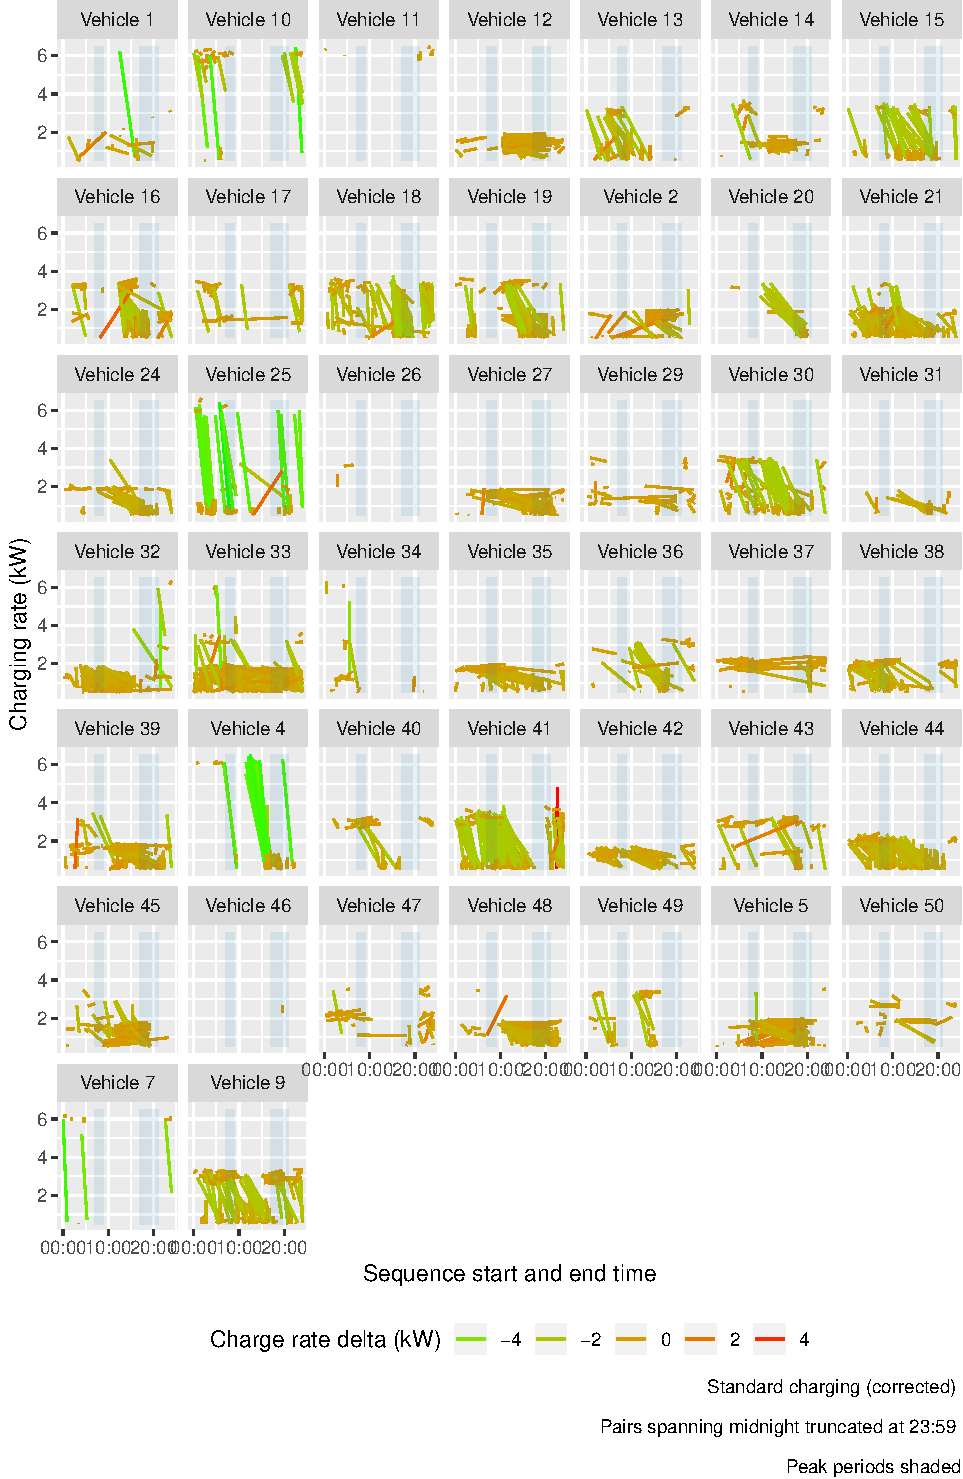
\includegraphics{/Users/ben/github/cfsOtago/evAnalysis/reports/fullReport/EVBB_report_EVBB_processed_all_v1.0_20180125_files/figure-latex/checkStdSequenceskW-1.pdf}
\caption{(\#fig:checkStdSequenceskW)Standard charging (corrected) - rate of charge}
\end{figure}

\begin{Shaded}
\begin{Highlighting}[]
\CommentTok{#ggsave("plots/standardChargePairs_kW_LineSegments.png", p, height = 10)}
\end{Highlighting}
\end{Shaded}

Figure @ref(fig:stdPowerDeltaDensity) shows the distribution of charge power deltas by peak/not peak period (of start time) for `standard' charge events. This suggests that the majority of charging events either hold power constant or decline over time with some sort of shoulder effect. A few increase. More of those which start in the `evening' and `not peak' period seem to hold the power level constant, presumably because the battery capacity is slightly lower at this time following day-time use.

\begin{Shaded}
\begin{Highlighting}[]
\NormalTok{p <-}\StringTok{ }\NormalTok{ggplot2}\OperatorTok{::}\KeywordTok{ggplot}\NormalTok{(dt, }\KeywordTok{aes}\NormalTok{(}\DataTypeTok{x =}\NormalTok{ chargePowerDelta, }\DataTypeTok{colour =}\NormalTok{ peakPeriod)) }\OperatorTok{+}
\StringTok{  }\KeywordTok{geom_density}\NormalTok{(}\DataTypeTok{alpha =} \FloatTok{0.5}\NormalTok{) }\OperatorTok{+}
\StringTok{  }\KeywordTok{guides}\NormalTok{(}\DataTypeTok{colour =} \KeywordTok{guide_legend}\NormalTok{(}\DataTypeTok{title =} \StringTok{"Peak period:"}\NormalTok{)) }\OperatorTok{+}
\StringTok{  }\KeywordTok{labs}\NormalTok{(}\DataTypeTok{x =} \StringTok{"Change in power from start to end (kW)"}\NormalTok{)}
\NormalTok{p}
\end{Highlighting}
\end{Shaded}

\begin{figure}
\centering
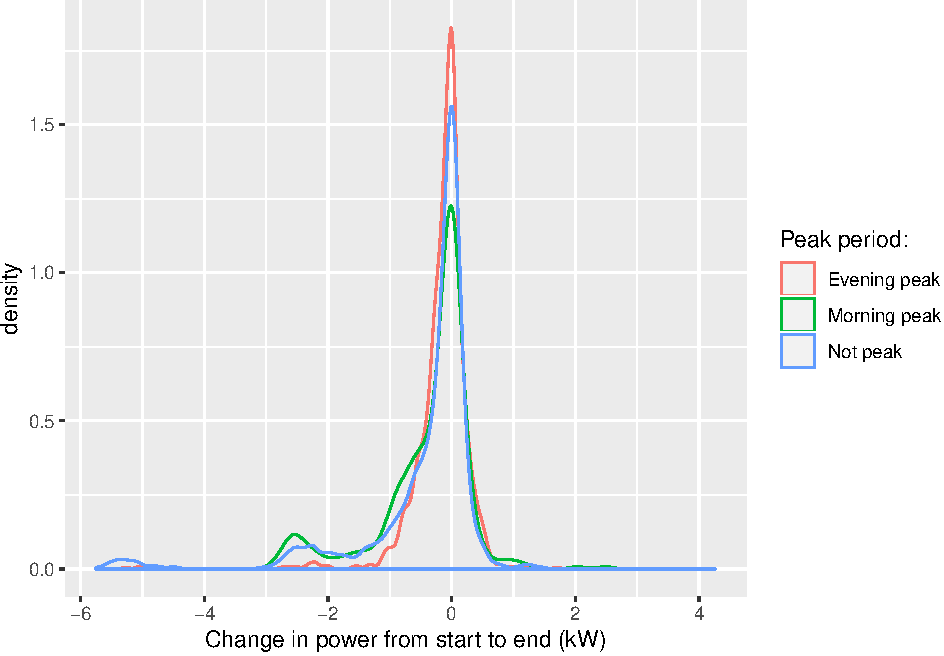
\includegraphics{/Users/ben/github/cfsOtago/evAnalysis/reports/fullReport/EVBB_report_EVBB_processed_all_v1.0_20180125_files/figure-latex/stdPowerDeltaDensity-1.pdf}
\caption{(\#fig:stdPowerDeltaDensity)Histogram of charge power deltas by peak/not peak period}
\end{figure}

Figure @ref(fig:checkStdSequencesSoC) uses the same approach but in this case the y value is charging rate (kW) at the start and end of the sequence. Colour (red end of the scale) is used to highlight pairs which show an `odd' pattern - e.g.~the battery state of charge decreased.

\begin{Shaded}
\begin{Highlighting}[]
\CommentTok{#dt <- dt[, SoC_pcDelta := SoC_pcDelta * -1] # invert so big drops become red in plot}
\NormalTok{p <-}\StringTok{ }\KeywordTok{makeSeqChargePlot}\NormalTok{(dt, }\DataTypeTok{y =} \StringTok{"startSoC_pc"}\NormalTok{, }
                       \DataTypeTok{yend =} \StringTok{"endSoC_pc"}\NormalTok{, }
                       \DataTypeTok{colour =}  \StringTok{"SoC_pcDelta"}\NormalTok{)}
\NormalTok{p <-}\StringTok{ }\NormalTok{p }\OperatorTok{+}\StringTok{ }
\StringTok{  }\KeywordTok{labs}\NormalTok{(}\DataTypeTok{y =} \StringTok{"State of charge (%)"}\NormalTok{,}
       \DataTypeTok{caption =} \StringTok{"Standard charging (corrected) }\CharTok{\textbackslash{}n}\StringTok{ Pairs spanning midnight truncated at 23:59"}\NormalTok{) }\OperatorTok{+}
\StringTok{  }\KeywordTok{guides}\NormalTok{(}\DataTypeTok{colour =} \KeywordTok{guide_legend}\NormalTok{(}\DataTypeTok{title =} \StringTok{"State of charge delta (%)"}\NormalTok{)) }\OperatorTok{+}
\StringTok{  }\KeywordTok{scale_color_continuous}\NormalTok{(}\DataTypeTok{low =} \StringTok{"red"}\NormalTok{, }\DataTypeTok{high =} \StringTok{"green"}\NormalTok{) }\CommentTok{# highlight ones that went down}
\NormalTok{yMin <-}\StringTok{ }\KeywordTok{min}\NormalTok{(dt}\OperatorTok{$}\NormalTok{startSoC_pc) }\CommentTok{# might not quite work if end is higher...}
\NormalTok{yMax <-}\StringTok{ }\KeywordTok{max}\NormalTok{(dt}\OperatorTok{$}\NormalTok{startSoC_pc) }\CommentTok{# might not quite work if end is higher...}
\KeywordTok{addPeaks}\NormalTok{(p)}
\end{Highlighting}
\end{Shaded}

\begin{figure}
\centering
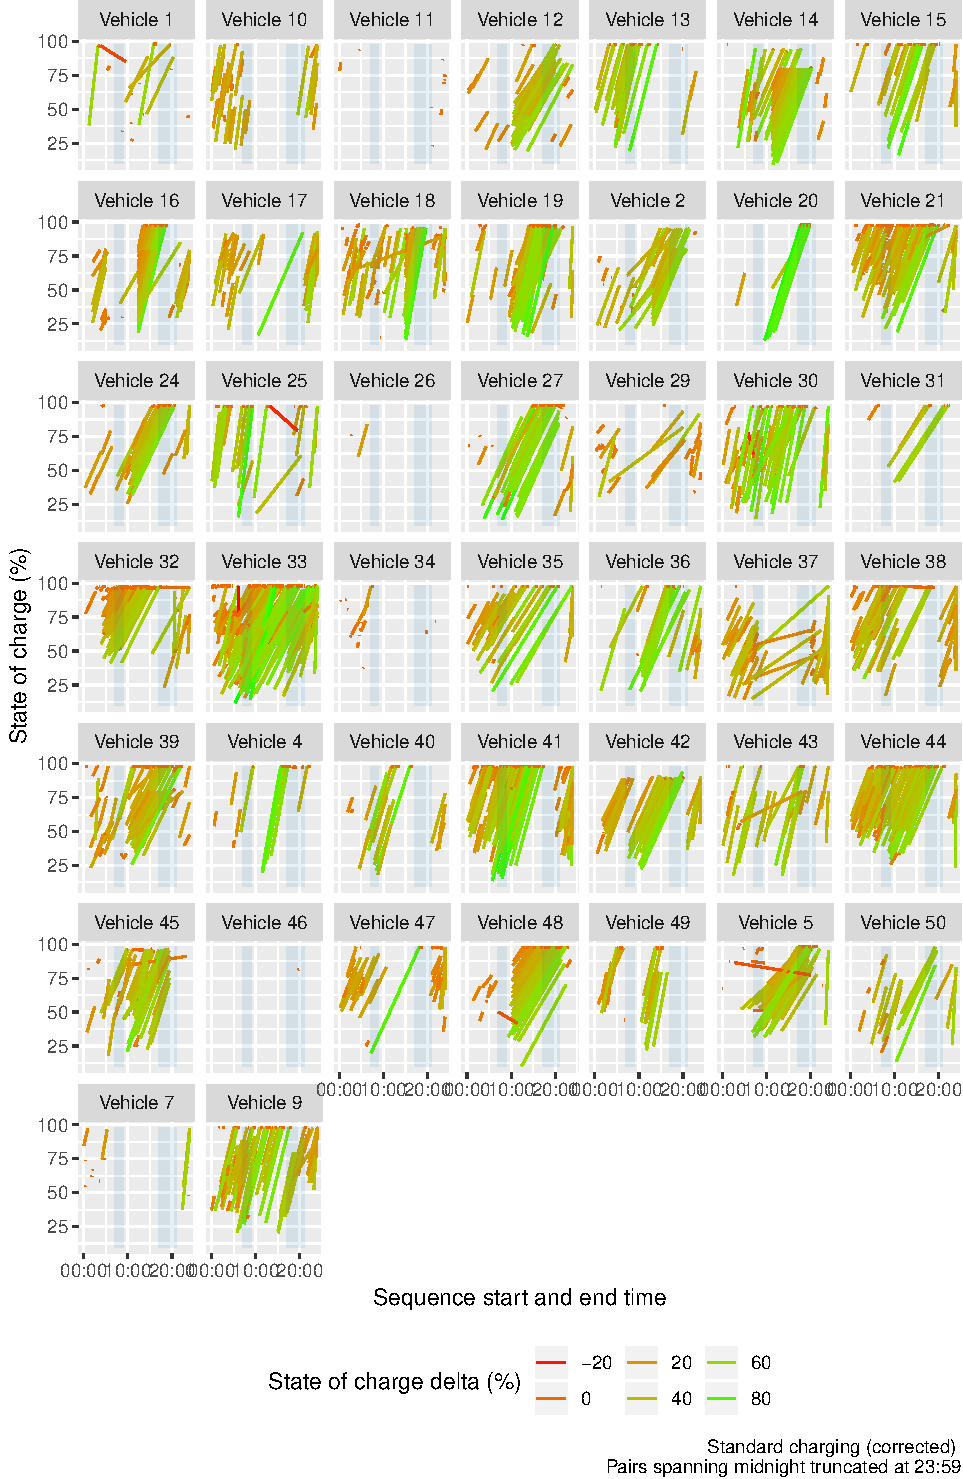
\includegraphics{/Users/ben/github/cfsOtago/evAnalysis/reports/fullReport/EVBB_report_EVBB_processed_all_v1.0_20180125_files/figure-latex/checkStdSequencesSoC-1.pdf}
\caption{(\#fig:checkStdSequencesSoC)Standard charging (corrected) - state of charge}
\end{figure}

\begin{Shaded}
\begin{Highlighting}[]
\CommentTok{#ggsave("plots/standardChargePairs_SoC_LineSegments.png", p, height = 10)}
\end{Highlighting}
\end{Shaded}

Figure @ref(fig:checkRapidSequenceskW) and Figure @ref(fig:checkRapidSequencesSoC) repeat these plots but for (corrected) `Rapid' charge events.

\begin{Shaded}
\begin{Highlighting}[]
\NormalTok{dt <-}\StringTok{ }\NormalTok{firstLastDT[chargeTypeCorrected }\OperatorTok\StringTok{ "Rapid"} \OperatorTok{&}\StringTok{ }
\StringTok{                    }\CommentTok{#startChargekW < 5 & #use this to filter out the few that seem to have 6kW chargers (or they might be 'Rapid' charging too)}
\StringTok{                    }\NormalTok{chargeFlag }\OperatorTok\StringTok{ "First"}\NormalTok{]}

\NormalTok{p <-}\StringTok{ }\KeywordTok{makeSeqChargePlot}\NormalTok{(dt, }\DataTypeTok{y =} \StringTok{"startChargekW"}\NormalTok{, }
                       \DataTypeTok{yend =} \StringTok{"endChargekW"}\NormalTok{, }
                       \DataTypeTok{colour =}  \StringTok{"chargePowerDelta"}\NormalTok{) }
\NormalTok{p <-}\StringTok{ }\NormalTok{p }\OperatorTok{+}\StringTok{ }
\StringTok{  }\KeywordTok{labs}\NormalTok{(}\DataTypeTok{y =} \StringTok{"Charging rate (kW)"}\NormalTok{,}
       \DataTypeTok{caption =} \StringTok{"Rapid charging (corrected) }\CharTok{\textbackslash{}n}\StringTok{ Pairs spanning midnight truncated at 23:59"}\NormalTok{) }\OperatorTok{+}
\StringTok{  }\KeywordTok{guides}\NormalTok{(}\DataTypeTok{colour =} \KeywordTok{guide_legend}\NormalTok{(}\DataTypeTok{title =} \StringTok{"Charge rate delta (kW)"}\NormalTok{)) }\OperatorTok{+}
\StringTok{  }\KeywordTok{scale_color_continuous}\NormalTok{(}\DataTypeTok{low =} \StringTok{"green"}\NormalTok{, }\DataTypeTok{high =} \StringTok{"red"}\NormalTok{) }\CommentTok{# highlight ones that went up}
\NormalTok{yMin <-}\StringTok{ }\KeywordTok{min}\NormalTok{(dt}\OperatorTok{$}\NormalTok{startChargekW) }\CommentTok{# might not quite work if end is higher...}
\NormalTok{yMax <-}\StringTok{ }\KeywordTok{max}\NormalTok{(dt}\OperatorTok{$}\NormalTok{startChargekW) }\CommentTok{# might not quite work if end is higher...}
\KeywordTok{addPeaks}\NormalTok{(p)}
\end{Highlighting}
\end{Shaded}

\begin{figure}
\centering
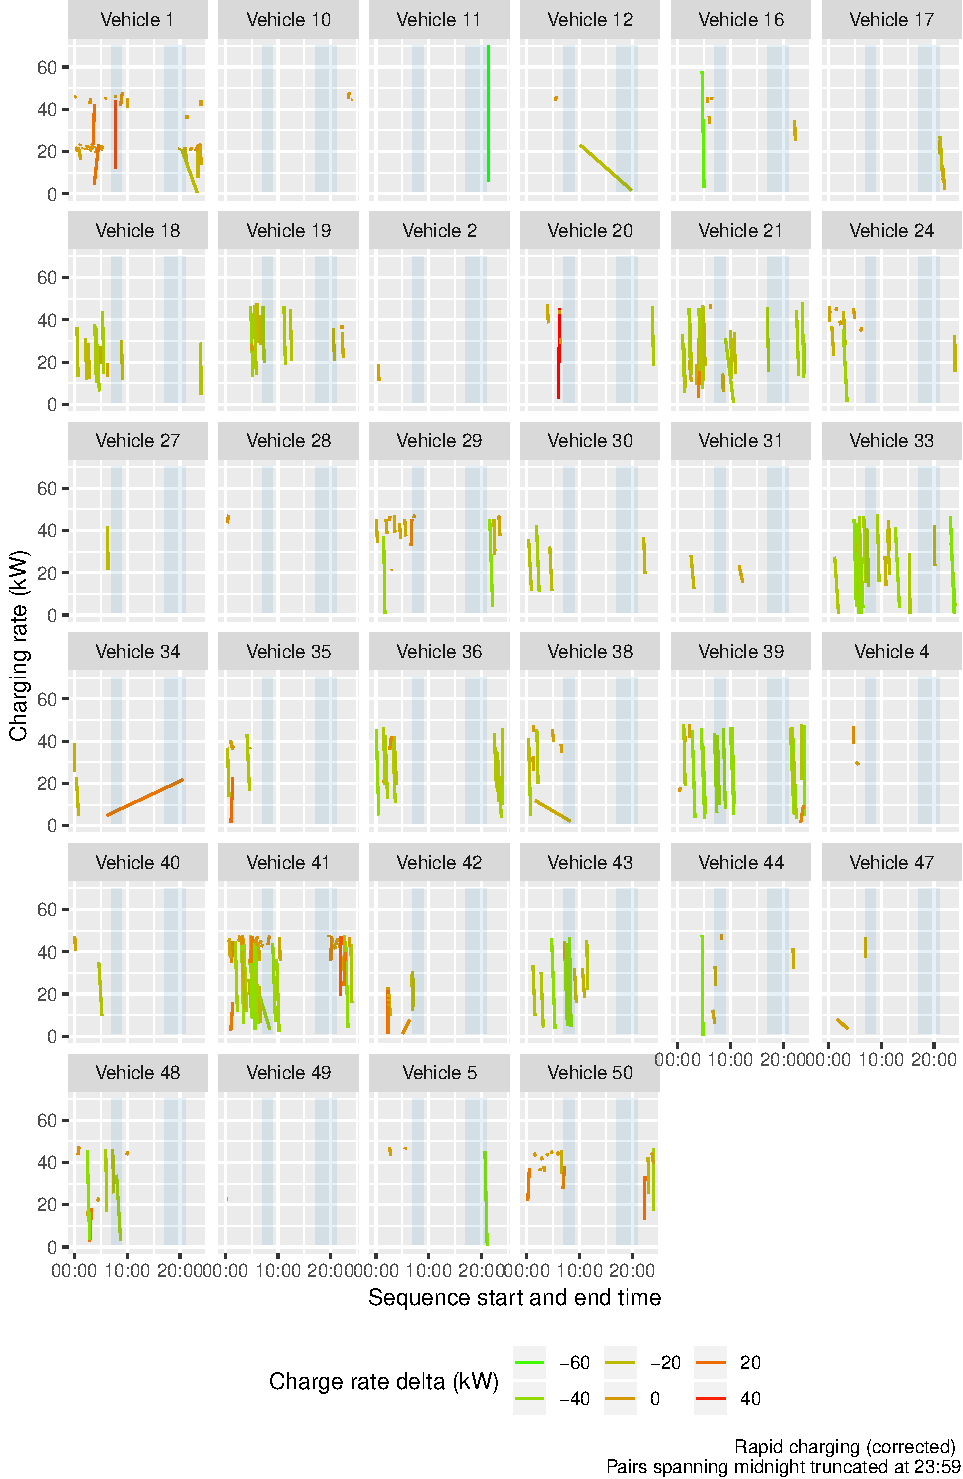
\includegraphics{/Users/ben/github/cfsOtago/evAnalysis/reports/fullReport/EVBB_report_EVBB_processed_all_v1.0_20180125_files/figure-latex/checkRapidSequenceskW-1.pdf}
\caption{(\#fig:checkRapidSequenceskW)Rapid charging (corrected) - rate of charge}
\end{figure}

\begin{Shaded}
\begin{Highlighting}[]
\CommentTok{#ggsave("plots/RapidChargePairs_kW_LineSegments.png", p, height = 10)}
\end{Highlighting}
\end{Shaded}

\begin{Shaded}
\begin{Highlighting}[]
\CommentTok{#dt <- dt[, SoC_pcDelta := SoC_pcDelta * -1] # invert so big drops become red in plot}
\NormalTok{p <-}\StringTok{ }\KeywordTok{makeSeqChargePlot}\NormalTok{(dt, }\DataTypeTok{y =} \StringTok{"startSoC_pc"}\NormalTok{, }
                       \DataTypeTok{yend =} \StringTok{"endSoC_pc"}\NormalTok{, }
                       \DataTypeTok{colour =}  \StringTok{"SoC_pcDelta"}\NormalTok{)}
\NormalTok{p <-}\StringTok{ }\NormalTok{p }\OperatorTok{+}\StringTok{ }
\StringTok{  }\KeywordTok{labs}\NormalTok{(}\DataTypeTok{y =} \StringTok{"State of charge (%)"}\NormalTok{,}
       \DataTypeTok{caption =} \StringTok{"Rapid charging (corrected) }\CharTok{\textbackslash{}n}\StringTok{ Pairs spanning midnight truncated at 23:59"}\NormalTok{) }\OperatorTok{+}
\StringTok{  }\KeywordTok{guides}\NormalTok{(}\DataTypeTok{colour =} \KeywordTok{guide_legend}\NormalTok{(}\DataTypeTok{title =} \StringTok{"State of charge delta (%)"}\NormalTok{)) }\OperatorTok{+}
\StringTok{  }\KeywordTok{scale_color_continuous}\NormalTok{(}\DataTypeTok{low =} \StringTok{"red"}\NormalTok{, }\DataTypeTok{high =} \StringTok{"green"}\NormalTok{) }\CommentTok{# highlight ones that went down}
\NormalTok{yMin <-}\StringTok{ }\KeywordTok{min}\NormalTok{(dt}\OperatorTok{$}\NormalTok{startSoC_pc) }\CommentTok{# might not quite work if end is higher...}
\NormalTok{yMax <-}\StringTok{ }\KeywordTok{max}\NormalTok{(dt}\OperatorTok{$}\NormalTok{startSoC_pc) }\CommentTok{# might not quite work if end is higher...}
\KeywordTok{addPeaks}\NormalTok{(p)}
\end{Highlighting}
\end{Shaded}

\begin{figure}
\centering
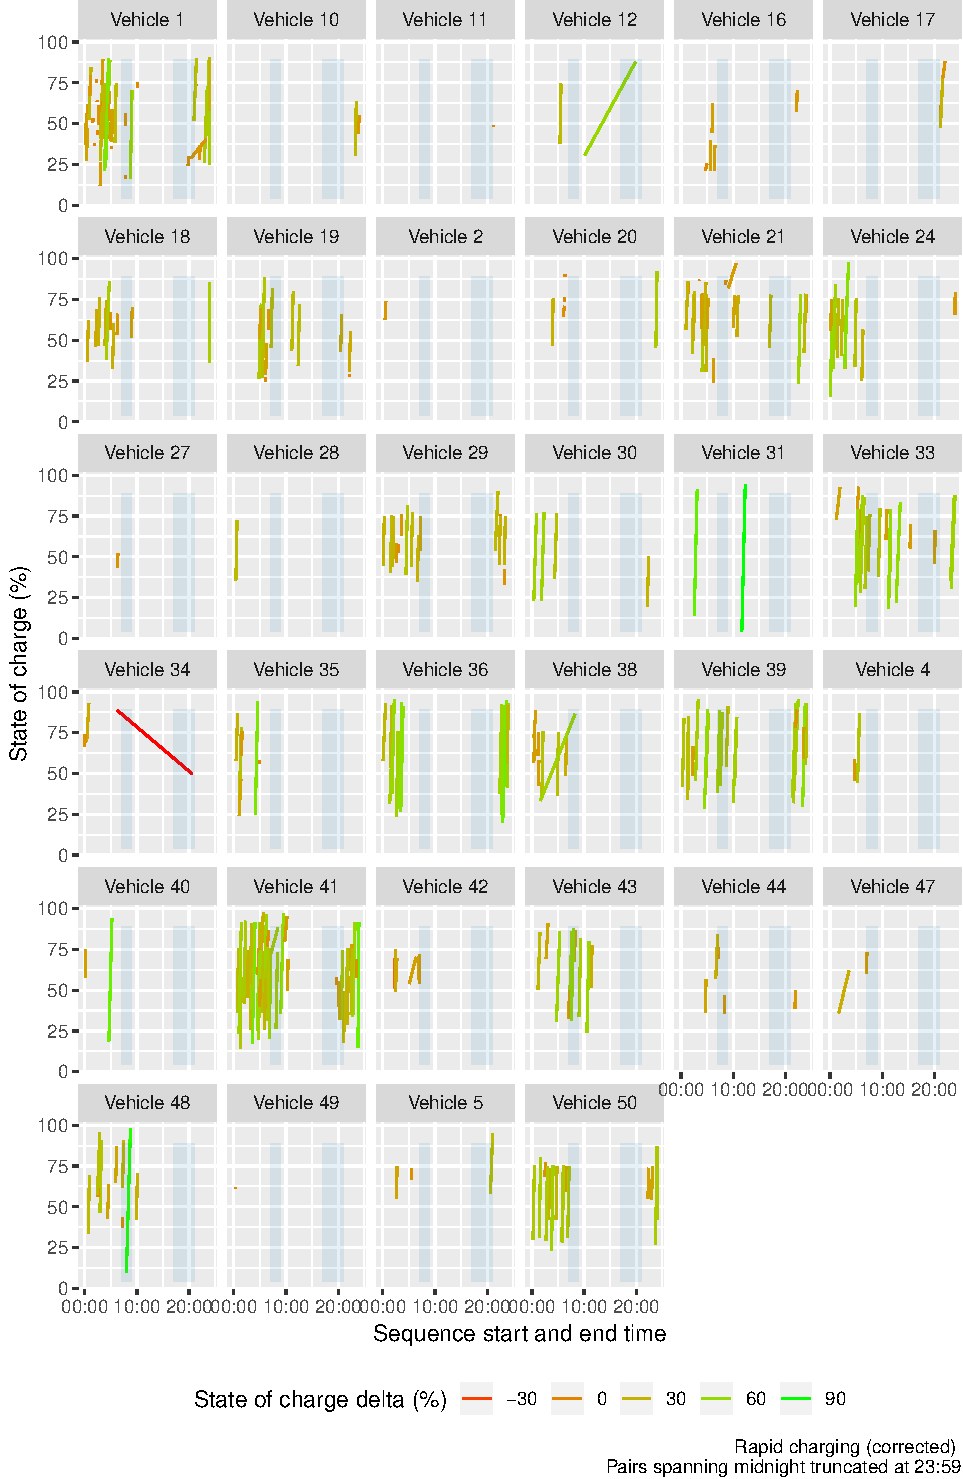
\includegraphics{/Users/ben/github/cfsOtago/evAnalysis/reports/fullReport/EVBB_report_EVBB_processed_all_v1.0_20180125_files/figure-latex/checkRapidSequencesSoC-1.pdf}
\caption{(\#fig:checkRapidSequencesSoC)Rapid charging (corrected) - state of charge}
\end{figure}

\begin{Shaded}
\begin{Highlighting}[]
\CommentTok{#ggsave("plots/RapidChargePairs_SoC_LineSegments.png", p, height = 10)}
\end{Highlighting}
\end{Shaded}

Figure @ref(fig:RapidPowerDeltaDensity) shows the distribution of charge power deltas by peak/not peak period (of start time) for all `Rapid' charge events. These show a rather different pattern.

\begin{Shaded}
\begin{Highlighting}[]
\NormalTok{p <-}\StringTok{ }\NormalTok{ggplot2}\OperatorTok{::}\KeywordTok{ggplot}\NormalTok{(dt, }\KeywordTok{aes}\NormalTok{(}\DataTypeTok{x =}\NormalTok{ chargePowerDelta, }\DataTypeTok{colour =}\NormalTok{ peakPeriod)) }\OperatorTok{+}
\StringTok{  }\KeywordTok{geom_density}\NormalTok{(}\DataTypeTok{alpha =} \FloatTok{0.5}\NormalTok{) }\OperatorTok{+}
\StringTok{  }\KeywordTok{guides}\NormalTok{(}\DataTypeTok{colour =} \KeywordTok{guide_legend}\NormalTok{(}\DataTypeTok{title =} \StringTok{"Peak period:"}\NormalTok{)) }\OperatorTok{+}
\StringTok{  }\KeywordTok{labs}\NormalTok{(}\DataTypeTok{x =} \StringTok{"Change in power from start to end (kW)"}\NormalTok{)}
\NormalTok{p}
\end{Highlighting}
\end{Shaded}

\begin{figure}
\centering
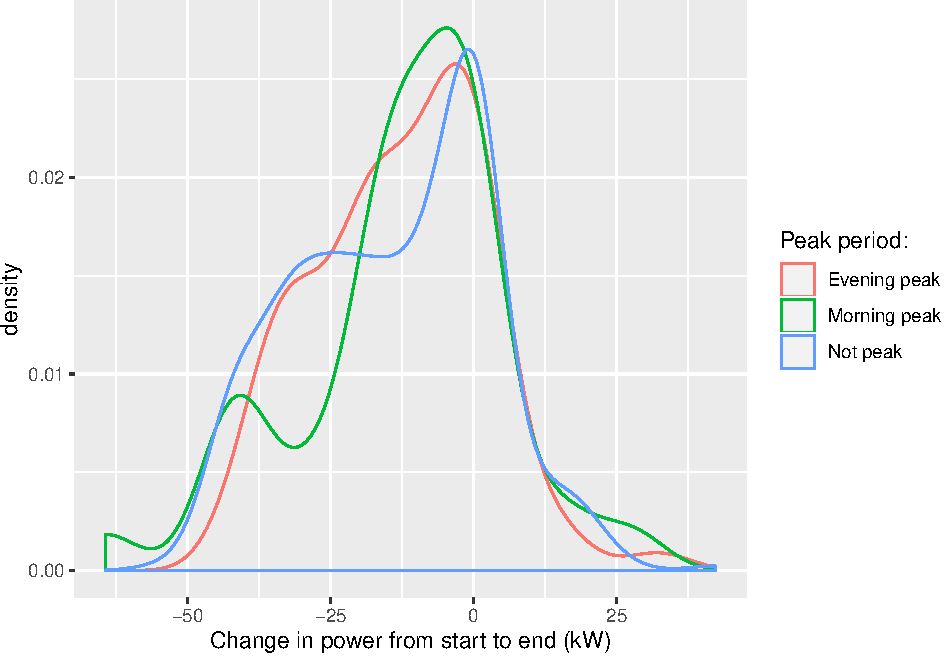
\includegraphics{/Users/ben/github/cfsOtago/evAnalysis/reports/fullReport/EVBB_report_EVBB_processed_all_v1.0_20180125_files/figure-latex/RapidPowerDeltaDensity-1.pdf}
\caption{(\#fig:RapidPowerDeltaDensity)Histogram of charge power deltas by peak/not peak period}
\end{figure}

\hypertarget{charge-type}{%
\subsubsection{Charge type}\label{charge-type}}

\texttt{chargeType} is used to classify charging events into standard vs rapid using the 7 kW threshold. But there may be misclassfications where a sequence starts on a rapid charger but power demand declines below the threshold. We can check this and have corrected it in some sections above using the start/end pairs.

\begin{Shaded}
\begin{Highlighting}[]
\CommentTok{# Check chargeType ----}

\NormalTok{t <-}\StringTok{ }\KeywordTok{table}\NormalTok{(firstLastDT}\OperatorTok{$}\NormalTok{chargeTypeError, firstLastDT}\OperatorTok{$}\NormalTok{chargeType, }\DataTypeTok{useNA =} \StringTok{"always"}\NormalTok{)}

\NormalTok{kableExtra}\OperatorTok{::}\KeywordTok{kable}\NormalTok{(t, }\DataTypeTok{caption =} \StringTok{"chargeType errors detected"}\NormalTok{) }\OperatorTok
\StringTok{  }\KeywordTok{kable_styling}\NormalTok{()}
\end{Highlighting}
\end{Shaded}

\begin{table}[t]

\caption{(\#tab:checkChargeType)chargeType errors detected}
\centering
\begin{tabular}{l|r|r|r|r}
\hline
  & Standard charging & Rapid charging & Not charging & NA\\
\hline
Error: first = Rapid, last = Standard & 0 & 60 & 0 & 0\\
\hline
Error: first = Standard, last = Rapid & 13 & 0 & 0 & 0\\
\hline
OK: first = Rapid, last = Rapid & 0 & 250 & 0 & 0\\
\hline
OK: first = Standard, last = Standard & 5704 & 0 & 0 & 0\\
\hline
NA & 5770 & 263 & 0 & 0\\
\hline
\end{tabular}
\end{table}

\begin{Shaded}
\begin{Highlighting}[]
\NormalTok{nError <-}\StringTok{ }\KeywordTok{nrow}\NormalTok{(firstLastDT[chargeTypeError }\OperatorTok\StringTok{ "Error"}\NormalTok{])}
\NormalTok{nErrorEVs <-}\StringTok{ }\KeywordTok{uniqueN}\NormalTok{(firstLastDT[chargeTypeError }\OperatorTok\StringTok{ "Error"}\NormalTok{]}\OperatorTok{$}\NormalTok{dvID)  }
\KeywordTok{message}\NormalTok{(}\StringTok{"There are "}\NormalTok{, nError, }\StringTok{" pairs (out of a total of "}\NormalTok{, }\KeywordTok{nrow}\NormalTok{(firstLastDT)}\OperatorTok{/}\DecValTok{2}\NormalTok{,}\StringTok{") from "}\NormalTok{, nErrorEVs ,}\StringTok{" EVs where charge type doesn't match."}\NormalTok{)}
\end{Highlighting}
\end{Shaded}

\begin{verbatim}
## There are 73 pairs (out of a total of 6030) from 23 EVs where charge type doesn't match.
\end{verbatim}

\hypertarget{references}{%
\section{References}\label{references}}


\end{document}
